\documentclass{beamer}
\usepackage{etex} % fixes new-dimension error

 % \usepackage{auto-pst-pdf}
\usepackage{xspace}
\usepackage{reotex}
\let\set\undefined

\definecolor{BrickRed}{rgb}{0.8, 0.25, 0.33}

%\usetheme{CambridgeUS}%{Copenhagen}%{Frankfurt}%{Singapore}%{CambridgeUS}
\usecolortheme[named=BrickRed]{structure} 
\useoutertheme[subsection=false]{miniframes}
\useinnertheme{circles}
%\useinnertheme[shadow=false]{rounded}
\setbeamertemplate{blocks}[rounded][shadow=false]

\setbeamercovered{transparent} 
\setbeamertemplate{navigation symbols}{} %Remove navigation bar
\setbeamertemplate{footline}[frame number] % add page number
\setbeamercolor{postit}{fg=BrickRed,bg=red!10}
\setbeamercolor{structure}{bg=black!10}
%\setbeamercolor{palette primary}{use=structure,fg=red,bg=green}
%\setbeamercolor{palette secondary}{use=structure,fg=red!75!black,bg=green}
\setbeamercolor{palette tertiary}{use=structure,bg=red!50!black,fg=white}
%\setbeamercolor{palette quaternary}{fg=black,bg=green}
%\setbeamercolor{normal text}{fg=black,bg=white}
%\setbeamercolor{block title alerted}{fg=red,bg=green}
%\setbeamercolor{block title example}{bg=black!10,fg=green}
\setbeamercolor{block body}{bg= black!5}

\setbeamercolor{block title alerted}{bg=red!25}
\setbeamercolor{block body alerted}{bg=red!10}

\setbeamercolor{block title example}{bg={rgb:green,2;black,1;white,5}}
\setbeamercolor{block body example}{bg={rgb:green,2;black,1;white,20}}

\usepackage{etex} % fixes new-dimension error
\usepackage{graphicx,amsmath}
\usepackage{stmaryrd} % cf. interleave
%\usepackage{./macros/myisolatin1}
%\usepackage{./macros/prooftree}
\usepackage{alltt}
%\usepackage{./macros/circle}
\usepackage{listings}
\usepackage{relsize} % relative size fonts
\usepackage{tikz}
\usetikzlibrary{%
  positioning
 ,patterns
 ,arrows
 ,calc
 ,shapes
 ,fit
 ,fadings
 ,decorations.pathreplacing
 ,plotmarks
% ,pgfplots.groupplots
 ,decorations.markings
}
% Nicer TT fonts
\usepackage[scaled=.83]{beramono}
\usepackage[T1]{fontenc}



%------ using eurosym -------------------------------------------------------
\usepackage{eurosym}
\def\inh#1{\mbox{\small\euro}_{#1}}
\def\eith#1#2{\mathopen{[}#1 \ ,#2\mathclose{]}}

%------ using xy ------------------------------------------------------------
\usepackage[all]{xy}
%\def\larrow#1#2#3{\xymatrix{ #3 & #1 \ar[l] _-{#2} }}
\def\larrow#1#2#3{\xymatrix{ #3 & #1 \ar[l] _--{#2} }}
\def\rarrow#1#2#3{\xymatrix{ #1 \ar[r]^-{#2} & #3 }}
\def\arLaw#1#2#3#4#5{
\xymatrix{
        #1      \ar@/^1pc/[rr]^-{#4} &
        #5 &
        #2      \ar@/^1pc/[ll]^-{#3}
}}
\def\arLeq#1#2#3#4{\arLaw{#1}{#2}{#3}{#4}\leq}
%------ using pstricks (rnode etc) ------------------------------------------
%\usepackage{pstricks,pst-node,pst-text,pst-3d}
%------ using color ---------------------------------------------------------
%\newrgbcolor{goldenrod}{.80392 .60784 .11373}
%\newrgbcolor{darkgoldenrod}{.5451 .39608 .03137}
%\newrgbcolor{brown}{.15 .15 .15}
%\newrgbcolor{darkolivegreen}{.33333 .41961 .18431}
\definecolor{goldenrod}{rgb}{.80392,.60784,.11373}
\definecolor{darkgoldenrod}{rgb}{.5451,.39608,.03137}
\definecolor{brown}{rgb}{.15,.15,.15}
\definecolor{darkolivegreen}{rgb}{.33333,.41961,.18431}
\definecolor{darkgreen}{rgb}{0,0.6,0}
%
%
\def\gold#1{{\textcolor{goldenrod}{#1}}}
\def\dgold#1{{\textcolor{darkgoldenrod}{#1}}}
%\def\brw#1{{\brown #1}}
\def\dkb#1{\textcolor{blue}{#1}}
\def\tdkb#1{\textbf{\textcolor{darkblue}{#1}}}
%%\def\gre#1{{\green #1}}
\def\gre#1{\textcolor{darkolivegreen}{#1}}
\def\gry#1{\textcolor{gray}{#1}}
\def\rdb#1{\textcolor{red}{#1}}
\definecolor{myGray}{gray}{0.85}
\def\laplace#1#2{*\txt{\mbox{ \fcolorbox{black}{myGray}{$\begin{array}{c}\mbox{#1}\\\\#2\\\\\end{array}$} }}}
\newenvironment{bluein}{\blue}{\black\hskip -2.5pt}

%------ contexts  ---------------------------------------------------------
\newcounter{prg}
\newenvironment{prg}[1]{\refstepcounter{prg}
\noindent
\textsc{\textbf{\arabic{prg}.}} \textsc{#1} } 
{\vspace{5mm}}

\newenvironment{sprg}[1]{
\noindent
\textsc{#1} }
{\vspace{3mm}}

\newcommand\blfootnote[1]{%
  \begingroup
  \renewcommand\thefootnote{}\footnote{#1}%
  \addtocounter{footnote}{-1}%
  \endgroup
}

\newtheorem{defi}{Defini\cao}[section]
\newtheorem{defi*}{Defini\cao}
\newtheorem{lema*}{Lema}
\newenvironment{lsbcom}
      {\footnotesize  \hrule ~\\ ~\\ {\bf \sc Nota:} }
      {\hrule  ~\\ ~\\  \normalsize}
      
\newenvironment{lsbcomi}
      {\footnotesize  \hrule ~\\ ~\\ {\bf \sc Note:} }
      {\hrule  ~\\ ~\\  \normalsize}
      
\newcommand{\fimdemo}{%
\raisebox{1.7mm}{\framebox[2mm]{\rule{0mm}{0mm}}}%
\hspace{-1.55mm}%
\rule{2mm}{0.5mm}%
\hspace{-0.45mm}%
\rule{0.5mm}{2mm}%
}

\newenvironment{intf}%
     {\traco}
    {\par \nopagebreak  \traco }
\newenvironment{demo}%
     {\vspace{-5mm}\noindent {\bf Prova:}}%
    {\par \nopagebreak  \noindent \fimdemo \vspace{3mm} }
\newenvironment{demoi}%
     {\vspace{-5mm}\noindent {\bf Proof:}}%
    {\par \nopagebreak  \noindent \fimdemo \vspace{3mm} }

\long\def\CUT#1{\relax}
\def\jnowarning#1{\typeout{Warning: #1 - document page [\thepage]}}

\newenvironment{slide}[1]{\begin{frame}\frametitle{#1}}{\end{frame}}
\long\def\marginproof#1#2{
\begin{slide}{Comments}
\footnotesize Proof of #1:\\\tiny#2
\end{slide}}

\long\def\margincomment#1{
\begin{slide}{Comments}
\footnotesize #1
\end{slide}}

\long\def\marginproof#1#2{\relax}
\long\def\margincomment#1{\relax}

\def\caixa#1{\medskip
  \begin{center}
  \fbox{\begin{minipage}{0.9\textwidth}\protect{#1}\end{minipage}}
  \end{center}}
  
  \def\caixam#1{\medskip
  \begin{center}
  \fbox{\begin{minipage}{0.9\textwidth}\protect{\vspace{-5mm}#1\vspace{-5mm}}\end{minipage}}
  \end{center}}
  
   \def\caixamm#1{\medskip
  \begin{center}
  \fbox{\begin{minipage}{0.9\textwidth}\protect{\vspace{-5mm}#1}\end{minipage}}
  \end{center}}

  
  \def\caixaaa#1{\medskip
  \begin{center}
  \fbox{\begin{minipage}{0.95\textwidth}\protect{#1}\end{minipage}}
  \end{center}}

\newcommand{\caixapeq}[2][0.71]{\medskip
  \fbox{\begin{minipage}{#1\textwidth}\protect{#2}\end{minipage}}}
  
  \def\caixapeqq#1{\medskip
  \fbox{\begin{minipage}{0.85\textwidth}\protect{#1}\end{minipage}}}
  
  \def\caixamin#1{
   \begin{center}
  \fbox{\begin{minipage}{0.70\textwidth}\protect{\vspace{-5mm}#1}\end{minipage}}
  \end{center}}


\def\endprf{\begin{flushright} $\Box$ \end{flushright} \vspace{3mm}}

%------ common jno, lab  ---------------------------------------------------------
%------------
\def\wider#1{~ #1 ~}
\def\altx#1#2{\mathopen{[}#1 \ ,#2\mathclose{]}}
\def\X{\end{document}}
\def\EXIT{ \bibliographystyle{plain} \bibliography{/Users/jno/share/texinputs/jno} \end{document}}
%------------
\def\fdep#1#2#3{#1 \mathbin{\stackrel{#2}{\rightarrow\/}} #3}
\def\lift#1{\stackrel.{#1}}
\newcommand{\N}{\mathbb{N}}
\newcommand{\Z}{\mathbb{Z}}
%\def\N{I\!\!N}                             % Nat numbers
%\def\Z{Z\!\!\!Z}                           % Integers
\def\real{I\!\!R}                           % Integers

\def\name#1{\makebox[15ex][l]{\emph{#1:}} &&}
\let\kons=\underline
\def\selup#1#2#3{#3^{#1}_{#2}}
\def\plus{\mathbin{\dagger}}
\def\asor{\mathbin{|}}                    % A | B
\def\enlist#1{\mathopen{[}#1\mathclose{]}} % [a,b,...z]
\def\from{\mathbin{\leftarrow}}
\def\listdef#1#2{\enlist{ ~ #1 \asor #2 \,}} % < f(x) | x <- l>
\def\into{\mathbin{\rightarrow}}
\let\seqdef=\listdef
\def\Seq#1{{#1}^{\star}}                 % X*
\def\f{\fun F}
\def\fuc#1{\mathsf {#1}}
\def\fun#1{\mathsf {#1}}
\def\g{\fun G}
\def\ff#1{\ap\f{#1}}
\def\gg#1{\ap\g{#1}}
\def\hfilleqn#1#2{\hfill$#1\arrayin{#2}$\hfill~}
\def\enset#1{\mathopen{ \{ }#1\mathclose{ \} }} % {a,b,...z}
\newcommand{\set}[1]{\left\{ #1 \right\}} % {a,b,...z}
\def\mcond#1#2#3{#1 \rightarrow #2,#3}
\def\bang{{!}}
\def\ap#1#2{#1\,#2}
\def\pow#1{\ap{{\cal P}}{(#1)}}           \def\pow#1{{\cal P}#1} % P(X) redefined
\def\unary#1#2{\def\arg{#2}\def\omisso{}\ifx\arg\omisso{\textsf{#1}}\else\ap{\textsf{#1}}{#2}\fi}
\def\card#1{\unary{card}{#1}}             % card 
\def\ker#1{\unary{ker}{#1}}  
\def\img#1{\unary{img}{#1}}
\def\st{\dot}
\def\len#1{\unary{len}{#1}}
\def\inds#1{\unary{inds}{#1}}
\def\dom#1{\unary{$\delta$}{#1}}
\def\rng#1{\unary{$\rho$}{#1}}
\let\ran=\rng
\def\issat{\mathbin\vdash}
\def\post#1{\hbox{post-}{#1}}              % post-#1
\def\pre#1{\hbox{pre-}{#1}}                % pre-#1
\def\presat{\mathbin{\issat_{pre}}}
\def\postsat{\mathbin{\issat_{post}}}
\def\laplace#1#2{*\txt{\fbox{$\begin{array}{c}\mbox{#1}\\\\#2\\\\\end{array}$}}}
\def\PF{{\cal PF}}
\def\ler#1{{\red \em [ read: #1]}}

\def\proj#1{\pi_{#1}}
%\def\deff{\stackrel{\rm def}{=}}          % Function definition symbol
\def\deff{\, :=\, }          % Function definition symbol
\def\setdef#1#2{\mathopen{\{} #1 \asor #2 \mathclose{\}}}
\def\asor{\mathbin{|}}                    % A | B
\def\p#1{\pi_{#1}}
\def\mvdep#1#2#3{#1 \mathbin{\stackrel{\rule[-.8ex]{0pt}{0pt}#2}{\rightharpoonup\hskip-1.5ex\rightharpoonup\/}} #3}
\def\gmvdep#1#2#3#4{#1 \mathbin{\stackrel{\rule[-.8ex]{0pt}{0pt}#2}{\rightharpoonup\hskip-1.5ex\rightharpoonup_{#4}\/}} #3}
\def\sshylo#1#2{\mean{~#1,#2~}}
\def\cata#1#2{\mathopen{(\!|}#1\mathclose{|\!)}_{{\fun #2}}}
\def\split#1#2{\const{#1,#2}}
\def\tuple#1{\mathopen{\langle}#1\mathclose{\rangle}} % <a,b,...z>
\def\divides{\mathbin{\setminus}}
\def\rdiv{\mathbin{\setminus}}
\def\ldiv{\mathbin{/}}
\def\true{\mathsf{true}}
\def\mean#1{\mathopen{[\![}#1\mathclose{]\!]}}
\def\false{\mathsf{false}}
\newenvironment{lcbr}{\left\{\begin{array}{l}}{\end{array}\right.}
\def\rcb#1#2#3#4{\def\nothing{}\def\range{#3}\mathopen{\langle}#1 \ #2 \ \ifx\range\nothing::\else: \ #3 :\fi \ #4\mathclose{\rangle}}

\def\rcbVdm#1#2#3#4{#1 \ #2 \ � #4}
\def\deffVdm{\mathbin{\raisebox{.2em}{\tiny \ \underline{$\mathchar"3234$} \ }}}
\def\mapVdm#1#2{#1 \mathbin{\tilde{\rightarrow}} #2}

\def\const#1{\mathopen{\langle}#1\mathclose{\rangle}} % <a,b,...z>
\def\comp{\mathbin{\cdot}}
\def\implied{\mathbin\Leftarrow}
\def\implies{\mathbin{\Rightarrow}}
\def\arrayin#1{\begin{array}{rcl}#1\end{array}}
\def\xarrayin#1{\begin{array}{cccccc}#1\end{array}}
\def\aspas#1{``#1''}
\def\ap#1#2{#1\,#2}
\def\unary#1#2{\def\arg{#2}\def\omisso{}\ifx\arg\omisso{\textsf{#1}}\else\ap{\textsf{#1}}{#2}\fi}
\def\card#1{\unary{card}{#1}}             % card x
\def\ker#1{\unary{ker}{#1}}  
\def\img#1{\unary{img}{#1}}
\def\ijust#1#2{&#1& \rule{2em}{0pt}  \{ \mbox{\rule[-.5em]{0pt}{1.2em} \footnotesize #2 \/} \}  \nonumber\\ && }
\def\just#1#2{\\\ijust{#1}{#2}}

\def\crflx#1{\Phi_{#1}}
\def\qcomp{\mathbin\bullet}
\def\xlarrow#1#2#3{\larrow{#3}{#2}{#1}} 
%\def\equiv{\Leftrightarrow}
\def\longlarrow#1#2#3{\xymatrix{ #3 && #1 \ar[ll] _-{#2} }}
%------------

%------  lsb  ---------------------------------------------------------

\def\drawit{\nccurve[angleA=-30,angleB=-150]{->}{NA}{NB}}

\def\cnext#1{\Circle_{#1}}
\def\clast#1{\Circle[f]_{#1}}
\def\calfut#1{\square_{#1}}

\def\mdepth#1{\mathsf{md}\, #1}

\def\always{\boxempty}
\def\eventual{\Diamond}
\def\nexts{\bigcirc}
\def\until{\mathbin{\mathcal U}}


\def\setFontSize#1{\gdef\currentFontSize{#1}\fontfamily{phv}\fontsize\currentFontSize\currentFontSize\selectfont}
\def\greybox#1{*\txt{\mbox{\fcolorbox{black}{myGray}{\mbox(40,15){#1}}}}}
\def\funbox#1{*\txt{\fcolorbox{white}{myGray}{\makebox(40,15){\black $#1$}}}}
\def\condition#1{*\txt{\fontfamily{phv}\fontsize\currentFontSize\currentFontSize\selectfont\pscirclebox[linecolor=white]{$#1$}}}
\def\checkpoint{*\txt{\pscirclebox*{}}}
\def\state{*\txt{\ovalnode[fillstyle=solid,fillcolor=red]{State}{\black Internal state}}}
\def\thing#1{$\bullet$ \rule{0pt}{.7cm} & \fcolorbox{black}{myGray}{#1}}

\def\const#1{\mathopen{\langle}#1\mathclose{\rangle}} % <a,b,...z>
\def\funbox#1{*\txt{\fcolorbox{white}{gray}{\makebox(40,15){\black $#1$}}}}
\def\pair#1{\const{#1}}
\def\bim{\fuc{B}}
%\def\abim#1{\bim\, #1}
\def\abim#1{\aapf{\bim}{#1}}
\def\bimm#1{\bim #1}
\def\iso{\cong}
\def\niso{\ncong}
\def\qcom{\mathbin{\boldsymbol{;}}}
\def\id{\fuc{id}}

\def\ainv#1{\overline{#1}}

\def\rsrt{\tau_{r}}   % right and left strength
\def\rsrtp#1{\tau_{r_{#1}}}   % right and left strength
\def\lsrt{\tau_{l}}

\def\igual{\mathbin{=}}
\def\dimp{\mathbin{\Leftrightarrow}}
\def\imp{\mathbin{\Rightarrow}}
\def\dimpp{\mathbin{\leftrightarrow}}
\def\impp{\mathbin{\rightarrow}}
\def\rimp{\mathbin{\Leftarrow}}
\def\limp{\mathbin{\multimap}}

\newcommand{\sse}{\mathbin{\, \operatorname{\textsf{iff}} \,}}
\def\e{\mathbin{\wedge}}
\def\ou{\mathbin{\vee}}

\def\aconv#1{#1^{\circ}} 
\newcommand{\fdec}[3]{#1: #2 \longrightarrow  #3}
\newcommand{\fdecf}[3]{#1: #2 \longrightarrow #3}
\newcommand{\fdef}[2]{#1\;=\; #2}

\newcommand{\adec}[3]{#1 \stackrel{#2}\longrightarrow #3}
\newcommand{\fblockf}[5]{
\begin{eqnarray*}
#1&\! \! \!: \!\! \!& #2 \longrightarrow #3\\
#1 & \! \!\! #4\, = \!\!\!& #5
\end{eqnarray*}
}

\newcommand{\sos}[3]{#3 \stackrel{#2}{\longleftarrow} #1}
\def\setcat{{\sf Set}}
\def\relcat{{\sf Rel}}
\def\parcat{{\sf Par}}
\def\predcat{{\sf Pred}}
\def\ordcat{{\sf Ord}}

\def\dois{\ensuremath{\boldsymbol{2}}}
\def\abv{\stackrel{\rm abv}{=}}
\def\sana#1{\mathopen{[\!(}#1\mathclose{)\!]}}
\def\deff{\triangleq} 
\def\pint{\mathbin{\interleave}}



% Fev 2010

\def\oculos{\mathbf{\bigcirc\!\! \frown\!\! \bigcirc}}
\def\ferramentas{\stackrel{\mathbf{\doublecap}}{\bigbox\!\!\bigbox}}
%\def\Act{\cal{N}}
\def\Act{N}

\def\vec#1{\Tilde{#1}}
\def\free#1{\textsf{free}(#1)}
\def\subs#1#2#3{\enset{#1/#2}\, #3}

\def\tim{\fuc{T}}
\def\att{\fuc{at}}
\def\md{\fuc{m}}

\def\bh#1#2{\apf{\ana{#1}}{#2}}

\def\apf#1#2{#1\; #2}                   % func applic no () -- f a
\def\appf#1#2{(#1\; #2)}                   % func applic with () -- (f a)
\def\aapf#1#2{#1 #2}                   % func applic no () -- f a

\def\aappf#1#2{(#1 #2)}                   % func applic with () -- (f a)
\def\appff#1#2{#1 (#2)}                   % func applic with () -- f(a)
%\def\ana#1#2{\mathopen{[\!(}#1\mathclose{)\!]}_{#2}}
%\def\ana#1#2{\mathopen{[\!(}#1\mathclose{)\!]}_{\fun #2}}
\def\ana#1{\mathopen{[\!(}#1\mathclose{)\!]}}
\def\sana#1{\mathopen{[\!(}#1\mathclose{)\!]}}

\def\iid#1{\id_{#1}}                     %  identitade default
\def\id{\mathbin{\fuc{id}}}    

\def\atim#1{\aapf{\tim}{#1}}
\def\final#1{\omega_{#1}}
\def\initial#1{\alpha_{#1}}

\def\ialg#1{\mu_{#1}}
\def\fcoalg#1{\nu_{#1}}
\def\hdd{\fun{hd}}
\def\tll{\fun{tl}}
\def\mrg{\fun{merge}}
\def\gnn{\fun{rep}}
\def\diag{\vartriangle}
\def\codiag{\triangledown}
\def\twist{\fun{twist}}
\def\swap{\fuc{s}}
\def\rtran#1{\stackrel{#1}{\longrightarrow}}
\def\tran#1{\stackrel{#1}{\longrightarrow}}
\def\primertran#1{\stackrel{#1}{\longrightarrow'}}
\def\rra{\longrightarrow}
\def\ppow{\ensuremath{\mathcal{P}}} 
\def\nx{\fun{next}}
\def\utran#1{\stackrel{#1}{\longrightarrow}}  % - a - > 
\def\reach#1{\stackrel{#1}{\longrightarrow}^*}

\newcommand{\blk}[1]{\mathbb{#1}}
\newcommand{\ger}[1]{\mathfrak{#1}}

\def\vs{\emph{vs}}
\def\ie{\emph{i.e.}}
\def\cf{\emph{cf.}}

\def\eg{\emph{e.g.}}

\def\PP{\blk{P}}

%------ CCS          -----------------------------------------%
\def\ppe{\mathbin{\vartriangleright}}
\def\kcomp{\mathbin{\boldsymbol{\bullet}}}
%\def\qcomp{\mathbin{\boldsymbol{;}}}
\def\ssp{\textsc{skip}}
\def\fim{\dagger}
%\def\ppe{\gg}
\def\cnil{\mathbf{0}}
\def\cpf#1#2{#1 . #2}                           % a.P
\def\cou#1#2{#1 \mathbin{+} #2}                 % P + Q
%\def\crt#1#2{\mathbin{#1 \setminus_{#2}}}       % P \ A
%\def\crtt#1#2{\mathbin{#1 \setminus\!\setminus_{#2}}}       % P \ A
%\def\crt#1#2{\mathsf{new}\, #2\;  #1}       % P \ A
\def\crt#1#2{#1 \backslash #2}       % P \ A
\def\crn#1#2{\{#2\}\, #1}                  % P[f]

%\def\crn#1#2{\mathbin{#1[#2]}}                  % P[f]
\def\couit#1#2{\Sigma_{#1}#2}                  %  + i=1,n
\def\cpar#1#2{#1 \mid #2}                       %  |
\def\ctpar#1#2{#1 \parallel #2}                       %  |
\def\cpars#1#2#3{#1 \mid_{#3} #2}               %  |S
\def\ffix#1#2{\underline{fix}~(#1\, =\, #2)}  % fix X
\def\fffix#1#2#3{\underline{fix}_{#1}~(#2\, =\, #3)}  % fix X
\def\tfix#1#2{\underline{\Tilde{fix}}~(\Tilde{#1}\, =\, \Tilde{#2})}  % fix X
%\def\ainv#1{\Bar{#1}}                   % ~ a
\def\ainv#1{\overline{#1}}                   % ~ a
\def\cif#1#2{\fuc{if}\, #1\, \fuc{then}\, #2}
\def\ccif#1#2#3{\fuc{if}\, #1\, \fuc{then}\, #2\, \fuc{else}\, #3}

\def\fres#1#2{#1 \restriction #2}                

\def\mean#1{\mathopen{[\![}#1\mathclose{]\!]}}
\def\llbracket{\mathopen{[\![}}
\def\rrbracket{\mathopen{]\!]}}

\def\cfree#1{\fuc{fn} (#1)}
\def\cbound#1{\fuc{bn} (#1)}
\def\anew#1{\overline{#1}\mathsf{new}\, } 
\def\transitatau{\rtran{\tau}}
\def\transitaa{\rtran{a}}


\def\cHat#1{{\cal T}(#1)}
\def\free#1{\textsf{free}(#1)}
\def\fuc#1{\textsf{#1}}
\def\subs#1#2#3{\enset{#1/#2}\, #3}
\def\PP{\blk{P}}
\def\PPf{\blk{P}_{\fim}}
\def\obs{\mathbin{\sim}}                     % P ~ Q
\def\nobs{\mathbin{\nsim}}                     % P ~ Q
\def\aobs{\mathbin{\approx}}                 % P ~ Q
\def\naobs{\mathbin{\not \approx}}                 % P ~ Q
\def\cobs{=}                                 % P = Q
\def\ssort#1{\blk{L}(#1)}                   % L()
\def\sysort#1{\blk{L}_s(#1)}                   % L()

\def\athen{\comp}
\def\PP{\blk{P}}

% 2015

\def\st{\mathbf{.}\,}
\def\laplace#1#2{*\txt{\mbox{ \fcolorbox{black}{myGray}{$\begin{array}{c}\mbox{#1}\\\\#2\\\\\end{array}$} }}}
\newcommand{\galois}[2]{#1\; \dashv\; #2}

\newcommand{\fddec}[3]{#1: #2 \longrightarrow  #3}

\def\mcrl{\textsf{mCRL2}}

\def\obs{\sim}
\def\eqm{\mathbin{\equiv}}                     
\def\noeqm{\mathbin{\not\!\equiv}}  
\newcommand{\flam}[2]{\lambda_{#1}\; .\; #2}
\def\existential#1#2{\exists_{#1}\;.\; #2}
\def\existencial#1#2{\exists_{#1}\;.\; #2}

\def\pv#1#2{\langle #1 \rangle\, #2}
\def\nc#1#2{[#1]\, #2}
\def\pvo#1#2{\langle \! \! \! \langle #1 \rangle \! \! \! \rangle\, #2}
\def\nco#1#2{\llbracket #1 \rrbracket #2}
\def\cvg#1{\llbracket \downarrow \rrbracket #1}
\def\cvgr#1#2{\llbracket #1 \downarrow \rrbracket #2}
\def\cvgl#1#2{\llbracket \downarrow  #1 \rrbracket #2}
\def\cvglr#1#2{\llbracket \downarrow  #1 \downarrow \rrbracket #2}
\def\lfp#1#2{\mu {#1}\, .\, {#2}}
\def\lpf#1#2{\mu {#1}\, .\, {#2}}
\def\gfp#1#2{\nu {#1}\, .\, {#2}}
\def\gpf#1#2{\nu {#1}\, .\, {#2}}
\def\mset#1{\vvv #1 \vvv}
\def\vvv{\vert \! \vert}
\def\mnc#1{\vvv [#1] \vvv}
\def\mpv#1{\vvv \langle #1 \rangle \vvv}
\def\bcomp#1{#1^{\text{c}}}
\def\eqm{\mathbin{\simeq}}
\def\noeqm{\mathbin{\not\!\simeq}}
\def\universal#1#2{\forall_{#1}\; .\; #2}
\def\existential#1#2{\exists_{#1}\; .\; #2}
\def\oexistential#1#2{\exists^{1}_{#1}\; .\; #2}

\def\reach#1{\stackrel{#1}{\longrightarrow}^*}


\def\rra{\longrightarrow}

\def\Lg#1{\mathsf{Lang}(#1)}
\def\Tr#1{\mathsf{Tr}(#1)}

\def\PP{\blk{P}}

\def\paths#1{\mathsf{Paths}(#1)}
\def\Mcomma{\text{ ,}}
\def\Msemicolon{\text{ ;}}
\def\Mdot{\text{ .}}


%%%%%%%%%%%%%%%% NUNO reconf

\def\reo{\textsf{Reo}\xspace}
\def\reolang{\textsf{CooPLa}\xspace}
\def\recoopla{\textsf{ReCooPLa}\xspace}
\def\CP{coordination pattern\xspace}
\def\CPs{coordination patterns\xspace}
\def\node#1{\ensuremath{\underline{#1}}}
\def\nameset{\ensuremath{\mathcal{I}}\xspace}
\def\endnameset{\ensuremath{\mathcal{E}}\xspace}
\def\nodeset{\ensuremath{\mathcal{N}}\xspace}
\def\portset{\ensuremath{\Sigma}\xspace}
\def\coordpatset{\ensuremath{\mathcal{P}}\xspace}
\def\logicmodel{\ensuremath{\mathcal{M}}\xspace}
\def\reconfset{\ensuremath{\mathcal{R}}\xspace}
\def\reconfoperationset{\ensuremath{\mathcal{O}}\xspace}
\def\channelset{\ensuremath{\mathcal{C}}\xspace}
\def\stateset{\ensuremath{\mathcal{S}}\xspace}
\def\typeset{\ensuremath{\mathcal{T}}\xspace}
\newcommand{\chanodesof}[2][\rho]{\ensuremath{\mathfrak{N}_{#1}^{#2}}\xspace}
\newcommand{\reconfop}{\ensuremath{\mathbin{\bullet}}}

\newcommand{\byreconfof}[1]{\ensuremath \stackrel{\rm #1}{\longleftarrow}}

\def\trans#1{\stackrel{#1}{\longrightarrow}}
\def\TS#1{\mathcal{G}(#1)}
\def\TSn#1{\mathcal{G}_{nodes}(#1)}


%%%%%%%%%%%%%%%%%%%%%%%%% ALEXANDRE
 \def\HHL{\mathcal{HHL}}
 
 \def\emskip{\vskip 1em}
 
 %%%%%%%%%%%%%%%%%%%%%% COMPONENTES NOV 2015
 \def\para{\mathbin{\boxtimes}}   % Mealy produto (sincrono)
\def\parc{\mathbin{\boxplus}}    % Mealy soma
\def\pars{\mathbin{\boxast}}     % Mealy misto
\def\shk#1#2{\bigl(#1\bigr)_{#2}}            % separated hook direita
\def\hk#1#2{#1\! \Lsh_{#2}}            % hook direita
\def\hkespaco#1#2{#1 \Lsh_{#2}}            % hook direita
%\def\feed#1{\Bigl( #1 \Bigr)\! \Lsh}            % hook direita
\def\feed#1{#1 \Lsh}            % hook direita
\def\kh#1#2{~_{#2}(#1)}           % hook esquerda

\def\flift#1{\ulcorner #1 \urcorner}           % funcoes embb
\def\singr#1{\lfloor #1 \rceil}

\def\pdiag{\bigtriangleup}      % diagonal em componentes
\def\pcodiag{\bigtriangledown}    % codiagonal em componentes

%\qcomp{\mathbin{\mathbf{;}}}
%\def\qcom#1#2{#1\qcomp#2}
%\def\sync{}  %d� problemas com o reotex.sty do Nuno Oliveria

 
 %%%%
 \def\SING{\ensuremath{\boldsymbol{1}}}
\def\ZERO{\ensuremath{\boldsymbol{0}}}

\def\ptran#1{\stackrel{#1}{\leadsto}}
\def\pptran#1#2{\stackrel{#1[#2]}{\leadsto}}

\def\bblue#1{\dkb{#1}}
\def\ctt#1{\underline{#1}}    
\def\lvazio{\fuc{nil}}   
\def\lcons{\mathbin{\fuc{cons}}} 
\def\either#1#2{[#1,#2]}
\def\att{\fun{at}}
\def\hd#1{\mathbin{\fuc{hd}} \, {#1}}              % hd x
\def\tl#1{\mathbin{\fuc{tl}} \, {#1}}   
\def\hdd{\mathbin{\fuc{hd}}}              % hd x
\def\tll{\mathbin{\fuc{tl}}}              % hd x\def\nnat{\blk{N}}
\def\rreal{\blk{R}}
\def\nnat{\blk{N}}
\def\vtran#1#2#3{#1\downarrow_{#3} #2 }
\def\labtran#1#2{~_{#1}\!\stackrel{#2}{\longleftarrow\, }}
\def\rabtran#1#2{\stackrel{#2}{\longrightarrow}_{#1}\, }
\def\excp#1{#1 + \SING}
\def\usplit#1#2{\langle #1, #2 \rangle}
\def\nnx{\fun{nx}}
\def\nxc{\ainv{\fun{nx}}}
%\def\ct{\fun{ct}}
%\def\ctc{\ainv{\fun{ct}}}
%\def\ini{\fun{ini}}
\def\nil{\underline{\fun{nil}}}
\def\att{\fun{at}}
\def\nx{\fun{next}}
\def\md{\fun{m}}
\def\acc{\ainv{\fun{ac}}}
\def\ac{\fun{ac}}
\newcommand{\mcar}[3]{(#1\, \rightarrow\, #2, \,   #3)}
\def\distr{\fuc{dr}}
\def\distl{\fuc{dl}}
\def\hdi#1{\mathbin{\fuc{last}} \, {#1}}              % hd x
\def\tli#1{\mathbin{\fuc{blast}} \, {#1}} 
\def\ip#1{\iota_{#1}}
\def\apf#1#2{#1\; #2}   
\def\m{\fuc{M}}

\def\onefuc{\fuc{Id}}
\def\triple#1{\const{#1}}
\def\kcomp{\mathbin{\boldsymbol{\bullet}}}  
 
\def\ntarrow{\Longrightarrow}
\newcommand{\ntdec}[3]{#1: #2 \ntarrow #3}
\def\ntiso{\stackrel{\iso}{\ntarrow}}

\def\rsrt{\tau_{r}}   % right and left strength
\def\rsrtp#1{\tau_{r_{#1}}}   % right and left strength
\def\lsrt{\tau_{l}}
\def\lsrtp#1{\tau_{l_{#1}}}   % right and left strength
\def\deltab{\delta}
\def\rpd{\delta_{r}}   % strength combination
\def\rpdp#1{\delta{r_{#1}}}
\def\lpd{\delta_{l}}
\def\ltrocam{\fuc{xl}_{+}}  % \assoc inv . \swap . \assoc
\def\rtrocam{\fuc{xr}_{+}}  
\def\dtrocam{\fuc{m}_{+}}  
\def\ltroca{\fuc{xl}}  % \assoc inv . \swap . \assoc
\def\rtroca{\fuc{xr}}  
\def\dtroca{\fuc{m}}  
\def\troca{\fuc{x}}  
\def\cat#1{{\sf #1}}
\def\flift#1{\ulcorner #1 \urcorner} 
\def\PR{\cat{Cp}}
\def\PRSp{\cat{Cp}_{Sp}}
\def\prcat#1{{\sf Cp_{#1}}}
%\newcommand{\prhom}[2]{\PR_{\bim}(#1, #2)}
\newcommand{\prhom}[2]{\PR(#1, #2)}
%\newcommand{\prhoms}[2]{\PR_{\bim}(#1, #2)_{Sp}}
\newcommand{\prhoms}[2]{\PR(#1, #2)_{Sp}}
\def\cid#1{\fuc{copy}_{#1}} 
\def\bismp#1{\sim{#1}}
\def\bism{\mathbin{\sim}}
\def\nbism{\overset{\bullet}{\sim}}
\def\nobism{\mathbin{\not\!\sim}}
\def\nilc{\fuc{nil}}
\def\idle{\fuc{idle}}
\def\inert#1{\fuc{inert}_{#1}}
\def\zerol{\fuc{zl}}
\def\zeror{\fuc{zr}}
\def\distr{\fuc{dr}}
\def\distl{\fuc{dl}}
\def\assoc{\fuc{a}}
\def\assocs{\fuc{a_*}}
\def\assocm{\fuc{a_+}}
\def\swap{\fuc{s}}
\def\swaps{\fuc{s_*}}
\def\swapm{\fuc{s_+}}
\def\lunit{\fuc{l}}
\def\runit{\fuc{r}}
\def\lunits{\fuc{l_*}}
\def\runits{\fuc{r_*}}
\def\lunitm{\fuc{l_+}}
\def\runitm{\fuc{r_+}}
\def\ana#1#2{\mathopen{[\!(}#1\mathclose{)\!]}_{#2}}
\def\sana#1{\mathopen{[\!(}#1\mathclose{)\!]}}
\def\bh#1#2{\apf{\ana{#1}}{#2}}
\def\BH{\cat{Bh}}
\def\diag{\vartriangle}
\def\codiag{\triangledown}
\def\psplit#1#2{\mathopen{\langle}#1, #2\mathclose{\rangle}}
\def\flift#1{\ulcorner #1 \urcorner} 
\def\rpdp#1{\delta{r_{#1}}}
\def\lpd{\delta_{l}}
%\def\lpdp#1{\lpd_{#1}}
\def\lpdp#1{\delta{l_{#1}}}

\def\bunit#1{\eta_{#1}}   % monad unit
\def\bmul#1{\mu_{#1}}   % monad multi

\def\bag#1{\fuc{Bag}_{#1}}

\newcommand{\MH}{\mathcal{H}}
\newcommand{\M}{M}
\newcommand{\Rz}{\textsc{T}}
\newcommand{\docircrlh}[2]{%
  \ooalign{$#1\rightarrow$\cr\hfil$#1\comp$\hfil\cr}}
\newcommand{\karrow}{\mathrel{\mathpalette\docircrlh\relax}}
\newcommand{\eqdef}{\widehat{=} \> \>}
\newcommand{\conc}{\> {\small \texttt{+} \hspace{-0.1cm} \texttt{+}} \>}
\newcommand{\mtime}{ [ 0, \infty ) }
\newcommand{\longerarrow}{\xrightarrow{\hspace*{1cm}}}
\newcommand{\klH}{\topo_{\MH}}
\newcommand{\topo}{{\bf Top}}
\def\hmul#1#2#3 { #1 \> \lhd \> #2 \> \rhd \> #3 }
\def\qcompp{\mathbin{\boldsymbol{;}}}
\def\qcom#1#2{#1\qcompp#2}


%--------------------
%--- by jose 2016 ---
%--------------------

\newcommand{\wrap}[1]{\begin{tabular}{@{}c@{}}#1\end{tabular}}
\newcommand{\mwrap}[1]{\ensuremath{\begin{array}{@{}c@{}}#1\end{array}}}
\newcommand{\myblock}[1]{\begin{beamercolorbox}[dp=1ex,center,rounded=true]%
  {postit} {\large \textbf{#1}} \end{beamercolorbox}}%
\def\trans#1{\xrightarrow{#1}}  % - a - > 

\newcommand{\frsplit}[3][.48]{
  \begin{columns}%[T] % align columns
  \begin{column}{#1\textwidth} #2 \end{column} ~~~
  \begin{column}{#1\textwidth} #3 \end{column} \end{columns}
}
\newcommand{\frsplitt}[3][.48]{
  \begin{columns}[T] % align columns
  \begin{column}{#1\textwidth} #2 \end{column} ~~~
  \begin{column}{#1\textwidth} #3 \end{column} \end{columns}
}
% rules
\newcommand{\typerule}[4][]{\ensuremath{\begin{array}[#1]{c}\textsf{\scriptsize ({#2})} \\#3 \\\hline\raisebox{-3pt}{\ensuremath{#4}}\end{array}}}
\newcommand{\styperule}[3][]{\ensuremath{\begin{array}[#1]{c} #2 \\[0.5mm]\hline\raisebox{-4pt}{\ensuremath{#3}}\end{array}}}
\newcommand{\shrk}{\vspace{-3mm}}


\newcommand{\evm}[1]{\langle #1 \rangle\,}
\newcommand{\alm}[1]{[#1]\,}


% Listing
\lstset{%language=Java
%  ,basicstyle=\footnotesize
  ,columns=space-fexible
%  ,numberstyle=\tiny
  ,mathescape=true
  ,showstringspaces=false
%  ,morekeywords={refract,global,local,on-change}
  ,morecomment=[l]{\%}
  ,commentstyle=\sl\sffamily\color{gray}\scriptsize
  ,basicstyle=\ttfamily\relsize{-0.5}
  ,keywordstyle=\bf\sffamily\color{purple}
%  ,emphstyle=\it\sffamily\color{blue!80!black}
  ,emphstyle=\bfseries\itshape\color{blue!80!black}
  ,emphstyle={[2]\itshape\color{red!70!black}}%\underbar}
  ,stringstyle=\color{darkgreen}
  ,alsoletter={-,||,+,<>}
  ,literate=*{->}{{{\color{red!70!black}$\to$}}}{1}
             {.}{{{\color{red!70!black}.}}}{1}
             {+}{{{\color{red!70!black}+}}}{1}
             {\#}{{{\color{red!70!black}\#}}}{1}
  ,emph={act,proc,init,sort}
  ,emph={[2]block,hide,comm,rename,allow,||,<>,sum}
%  ,emphstyle={[2]\color{blue}}2
  ,framerule=1pt
  ,backgroundcolor=\color{black!2}
  ,rulecolor=\color{black!30}
  ,frame=tblr
  ,xleftmargin=4pt
  ,xrightmargin=4pt
  ,captionpos=b
%  ,belowcaptionskip=\medskipamount
  ,aboveskip=\baselineskip
  ,floatplacement=htb
}
\lstdefinestyle{bash}{literate=*}
\newcommand{\code}[1]{\lstinline[basicstyle=\ttfamily\relsize{-0.5},keywordstyle=\bf\sffamily\color{purple},columns=fullflexible,keepspaces]�#1�}
\newcommand{\mcode}[1]{\text{\code{#1}}}
\newcommand{\bash}[1]{\lstinline[basicstyle=\ttfamily\relsize{-0.5}\color{darkgreen},keywordstyle=\bf\sffamily\color{purple},columns=fullflexible,keepspaces]�#1�}





\title{
	Introduction to modal logic
	}
\author{Jos\'e Proen\c{c}a}
\institute{HASLab - INESC TEC \\ Universidade do Minho\\ Braga, Portugal}

\date{
\begin{tabular}{c}
\\
    Mar\c{c}o, 2016
\end{tabular}
}

\begin{document}

\frame[plain]{\titlepage}

\section{What's in a logic?}


%----------------------------------------------------------------------------------
\begin{slide}{A logic}\label{s:1}
\small
\begin{block}{A language}
i.e. a collection of well-formed expressions to which meaning can be assigned.
\end{block}
\begin{block}{A semantics}
describing how language expressions are interpreted as statements about something.
\end{block}
\begin{block}{A deductive system}
i.e. a collection of rules to derive in a purely syntactic way facts and relationships among semantic objects described in the language.
\end{block}

\begin{block}{Note}
\begin{itemize}
\item a purely syntactic approach (up to the 1940's; the \dgold{sacred form})
\item a model theoretic approach (A. Tarski legacy)
\end{itemize}
\end{block}

\end{slide}


%----------------------------------------------------------------------------------
\begin{slide}{Semantic reasoning: models}\label{s:2}
\small
\begin{itemize}
\item \dgold{sentences}
\item \dgold{models} \& \dgold{satisfaction}: $\ger{M} \models \phi$
\item \dgold{validity}: $\models \phi$ ($\phi$ is satisfied in every possible structure)
\item \dgold{logical consequence}: $\Phi \models \phi$ ($\phi$ is satisfied in every model of $\Phi$)
\item \dgold{theory}: $Th\, \Phi$ (set of logical consequences of a set of sentences $\Phi$)
\end{itemize}

\end{slide}


%----------------------------------------------------------------------------------
\begin{slide}{Syntactic reasoning: deductive systems}\label{s:3}
\small

\begin{block}{Deductive systems $\vdash$}
\begin{itemize}
\item sequents
\item Hilbert systems
\item natural deduction
\item tableaux systems
\item resolution
\item $\cdots$
\end{itemize}
\end{block}


\begin{flushright}
\begin{itemize}
\item \dgold{derivation} and \dgold{proof}
\item \dgold{deductive consequence}: $\Phi \vdash \phi$
\item \dgold{theorem}: $\vdash \phi$
\end{itemize}
\end{flushright}

\end{slide}

%----------------------------------------------------------------------------------
\begin{slide}{Soundness \& completeness}\label{s:4}
\small

\begin{itemize}
\item A deductive system $\vdash$ is \dgold{sound} wrt a semantics $\models$ if for all sentences $\phi$
$$ \vdash \phi\; \; \Longrightarrow\; \; \models \phi$$
\begin{flushright}
(\dgold{every theorem is valid})
\end{flushright}
\item $\cdots$ \dgold{complete} ...
$$ \models \phi\; \;  \Longrightarrow\; \;  \vdash \phi$$
\begin{flushright}
(\dgold{every valid sentence is a theorem})
\end{flushright}
 \end{itemize}

\end{slide}





%----------------------------------------------------------------------------------
\begin{slide}{Consistency \& refutability}\label{s:5}
\small

For logics with \dgold{negation} and a \dgold{conjunction} operator

\begin{itemize}
\item A sentence $\phi$ is \dgold{refutable} if $\neg \phi$ is a theorem (i.e. $\vdash \neg \phi$)
\item A set of sentences $\Phi$ is \dgold{refutable} if some finite conjunction of elements in $\Phi$ is refutable
\item $\phi$ or $\Phi$ is \dgold{consistent} if it is not refutable.
\end{itemize}

\end{slide}

%----------------------------------------------------------------------------------
\begin{slide}{Examples}\label{s:6}
\small

$$ \dgold{\ger{M}} \models \dkb{\phi} $$

\begin{itemize}
\item Propositional logic (logic of \dkb{uninterpreted assertions}; models are \dgold{truth assignments})
\item Equational logic (formalises \dkb{equational} reasoning; models are \dgold{algebras})
\item First-order logic (logic of \dkb{predicates} and \dkb{quatification} over structures; models are \dgold{relational structures})
\item Modal logics 
\item ...
\end{itemize}

\end{slide}

\section{Modal Logic}


%----------------------------------------------------------------------------------
\begin{slide}{Modal logic (from P. Blackburn, 2007)}\label{s:9}
\small
\emph{Over the years modal logic has been applied in many different ways. It has been used as a tool for reasoning about \dgold{time, beliefs, computational systems, necessity} and \dgold{possibility}, and much else besides. \\
~\\

These applications, though diverse, have something important in common: the key ideas they employ (flows of time, relations between epistemic alternatives, transitions between computational states, networks of possible worlds) can all be represented as \dgold{simple graph-like structures}.  }
~\\
~\\

Modal logics are
\begin{itemize}
\item  \dgold{tools to talk about relational, or graph-like structures}.
\item  \dgold{fragments of classical ones}, with restricted forms of quantification ...
\item  ... which tend to be \dgold{decidable} and described in a pointfree notations.
\end{itemize}
\end{slide}



%----------------------------------------------------------------------------------
\begin{slide}{The language}\label{s:10}
\small
\begin{block}{Syntax}
\begin{equation*}
\phi\; ::=\; p \: \mid\: \true\: \mid\: \false\: \mid\: \neg \phi \: \mid\: \phi_1 \e \phi_2\: \mid\:
           \phi_1 \impp  \phi_2\:   \mid\:
           \pv{m}{\phi} \:  \mid\:
           \nc{m}{\phi} 
\end{equation*}
where $p \in \dgold{\mathsf{PROP}}$ and $m \in \dkb{\mathsf{MOD}}$
\end{block}
\vspace{1cm}

Disjunction ($\ou$) and equivalence ($\dimpp$) are defined by abbreviation.
The \structure{signature} of the basic modal language is determined by sets $\dgold{\mathsf{PROP}}$ of \dgold{propositional} symbols (typically assumed to be denumerably infinite) and $\dkb{\mathsf{MOD}}$ of \dkb{modality} symbols.
\end{slide}

%----------------------------------------------------------------------------------
\begin{slide}{The language}\label{s:11}
\small
\begin{block}{Notes}
\begin{itemize}
\item if there is only one modality in the signature (i.e., $\mathsf{MOD}$ is a singleton), write simply \dgold{$\eventual \phi$} and \dgold{$\always \phi$}
\item the language has some redundancy: in particular modal connectives are \dgold{dual} (as quantifiers are in first-order logic):
$\nc{m}{\phi}$ is equivalent to  $\neg \pv{m}{\neg \phi}$
\item define \dgold{modal depth} in a formula $\phi$, denoted by \dgold{$\mdepth{\phi}$} as the maximum level of nesting of modalities in $\phi$
\end{itemize}
\end{block}

\begin{exampleblock}{Example}
  Models as LTSs over Act.\\
  $\dkb{MOD} = \blk P {Act}$ -- sets of actions.\\
  $\pv{\dkb{\set{a,b}}} \phi$ can be read as ``\emph{after observing $a$
\dgold{or} $b$, $\phi$ must hold.}''\\
  $\nc{\dkb{\set{a,b}}} \phi$ can be read as ``\emph{after observing $a$ \dgold{and} $b$, $\phi$ must hold.}''
\end{exampleblock}

\end{slide}

%----------------------------------------------------------------------------------
\begin{slide}{Semantics}\label{s:12}

\myblock{$\ger{M}, w ~\models~ \phi$  ~~--~~what does it mean? }

\begin{block}{Model definition}
A \dkb{model} for the language is a pair $\dkb{\ger{M}} = \pair{\ger{F},V}$, where
\begin{itemize}
\item $\ger{F} = \pair{\dgold{W}, \enset{\alert{R_m}}_{m \in \mathsf{MOD}}}$  \\ is a \dkb{Kripke frame}, ie, a non empty set \dgold{$W$} and a family \alert{$R_m$} of \alert{binary relations} (called \emph{accessibility relations})
over \dgold{$W$}, one for each modality symbol $m \in \mathsf{MOD}$. Elements of \dgold{$W$} are called \dgold{points},  \dgold{states},  \dgold{worlds} or
simply  \dgold{vertices} in  directed graphs. 
\item $\fdec{V}{\mathsf{PROP}}{\pow{(W)}}$ is a \dkb{valuation}.
\end{itemize}
\end{block}


\begin{exampleblock}{When MOD = \textbf{1}}
\begin{itemize}
  \item \dgold{$\eventual \phi$} and \dgold{$\always \phi$} instead of
        \dkb{$\pv{\cdot} \phi$} and \dkb{$\nc{\cdot} \phi$}
  \item \dgold{$\ger{F} = \pair{W,R}$} instead of
        \dkb{$\ger{F} = \pair{{W}, \enset{{R_m}}_{m \in \mathsf{MOD}}}$}
\end{itemize}
\end{exampleblock}
\end{slide}


%----------------------------------------------------------------------------------
\begin{slide}{Semantics}\label{s:13}
\small
\begin{block}{Safistaction: for a model $\ger{M}$ and a point $w$}
\begin{align*}
\ger{M}, w & \models \true &&\\
\ger{M}, w & \not \models  \false &&\\
\ger{M}, w & \models  p &  \text{~~~ \textsf{iff} ~~~}  & w \in V(p)\\
\ger{M}, w  & \models \neg \phi  & \text{~~~ \textsf{iff} ~~~} & \ger{M}, w  \not \models \phi \\
\ger{M}, w & \models \phi_1 \e \phi_2  &\text{~~~ \textsf{iff} ~~~} & \ger{M}, w \models  \phi_1 \;\; \text{and}\;\;
                                                   \ger{M}, w \models  \phi_2 \\
\ger{M}, w & \models \phi_1 \impp \phi_2 & \text{~~~ \textsf{iff} ~~~} & \ger{M}, w \not \models \phi_1  \;\; \text{or}\;\; 
                                                  \ger{M}, w \models \phi_2 \\
%\ger{M}, w  &\models \phi_1 \ou \phi_2 \text{~~~ \textsf{iff} ~~~} E \models \phi_1 \;\; \ou\;\;
%                                                   E \models \phi_2 \\
\ger{M}, w  &\models \pv{m}{\phi} & \text{ ~~~ \textsf{iff} ~~~} &
\text{there exists}\; v \in W \;\text{st}\; w R_m v\; \text{and}\; \ger{M}, v \models \phi\\
\ger{M}, w & \models \nc{m}{\phi} & \text{~~~ \textsf{iff} ~~~} &
\text{for all}\; v \in W \; \text{st}\; w R_m v\; \text{and}\; \ger{M}, v \models \phi\\
\end{align*}
\end{block}
\end{slide}


%----------------------------------------------------------------------------------
\begin{slide}{Semantics}\label{s:14}
\small
\begin{block}{Satisfaction}
A formula $\phi$ is
\begin{itemize}
\item \dgold{satisfiable in a model}  $\ger{M}$ if it is satisfied at some point of $\ger{M}$
\item \dgold{globally satisfied} in $\ger{M}$ ($\ger{M} \models \phi$) if it is satisfied at all points in $\ger{M}$
\item \dgold{valid} ($\models \phi$) if it is globally satisfied in all models
\item \dgold{a semantic consequence} of a set of formulas $\Gamma$ ($\Gamma \models \phi$) if for all models $\ger{M}$ and all
points $w$, if $\ger{M}, w \models \Gamma$ then $\ger{M}, w \models \phi$
\end{itemize}
\end{block}
\end{slide}


%----------------------------------------------------------------------------------
\begin{slide}{Example: Hennessy-Milner logic}\label{s:17}
\small
\begin{block}{Process logic (\dgold{Hennessy-Milner logic})}
\begin{itemize}
\item $\mathsf{PROP} = \emptyset$
\item $W = \PP$ is a set of states, typically process terms, in a labelled transition system 
\item each subset $K \subseteq Act$ of actions generates a modality corresponding to transitions labelled by an element of $K$ 
\end{itemize}
\end{block}
Assuming the underlying LTS \dgold{$\ger{F} = \pair{\PP, \setdef{p \tran{K} p'}{K \subseteq Act}}$} as the modal frame, satisfaction is abbreviated as
\begin{align*}
p & \models \pv{K}{\phi} \text{ ~~~~~~~~ \textsf{iff} ~~~}
\existential{q \in \setdef{p'}{p \tran{a} p' \; \e\;  a \in K}}{q \models \phi} \\
p & \models \nc{K}{\phi} \text{~~~~~~~~~~ \textsf{iff} ~~~}
\universal{q \in \setdef{p'}{p \tran{a} p' \; \e\;  a \in K}}{q \models \phi} 
\end{align*}
\end{slide}

\begin{slide}{Example: Hennessy-Milner logic}
\small

\begin{columns}
\column{0.38\textwidth}
\centering
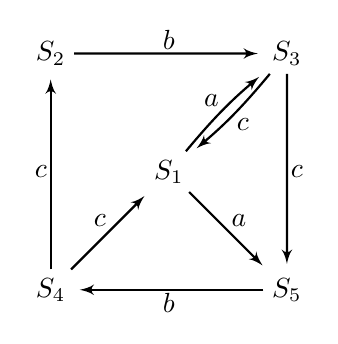
\begin{tikzpicture}[scale=1.5,%
  every node/.style={auto,inner sep=1pt},%
  every edge/.style={draw, thick,-latex',shorten >= 2pt}]
\tikzstyle{n} = [inner sep=3pt]
\node[n](s2)at(0,2){$S_2$};
\node[n](s3)at(2,2){$S_3$};
\node[n](s1)at(1,1){$S_1$};
\node[n](s5)at(0,0){$S_4$};
\node[n](s4)at(2,0){$S_5$};
\draw[->]
  (s1)edge node{$a$}(s4) edge[bend left=5pt] node{$a$}(s3)
  (s2)edge node{$b$}(s3)
  (s3)edge node{$c$}(s4) edge[bend left=5pt] node{$c$}(s1)
  (s4)edge node{$b$}(s5)
  (s5)edge node{$c$}(s2) edge node{$c$}(s1);
\end{tikzpicture}

\column{0.58\textwidth}
\begin{exampleblock}{Prove:}
\begin{enumerate}
  \item $S_2 \models \alm a (\evm b tt \land \evm c tt)$\\
  \item $S_1 \not \models \alm a(\evm b tt \land \evm c tt)$\\
  \item $S_2 \models \alm b \alm c(\evm a tt \lor \evm b tt)$\\
  \item $S_1 \models \alm b \alm c(\evm a tt \lor \evm b tt)$    
%  \item $S_2 \models [a](⟨b⟩tt ∧ ⟨c⟩tt)$\\
%  \item $S_1 \not \models [a](⟨b⟩tt ∧ ⟨c⟩tt)$\\
%  \item $S_2 \models [b][c](⟨a⟩tt ∨ ⟨c⟩tt)$\\
%  \item $S_1 \models [b][c](⟨a⟩tt ∨ ⟨c⟩tt)$    
\end{enumerate}
\end{exampleblock}
\end{columns}
  
\end{slide}

%----------------------------------------------------------------------------------
\begin{slide}{Proof system $\mathbf{K}$}\label{s:37}
\small

\begin{block}{Minimal modal logic}

\begin{itemize}
\item all formulas with the form of a \dgold{propositional tautology} (including formulas which contain  modalities 
but are truth-functionally tautologous) 
\item all instances of  the axiom schema:
\begin{equation*}
\always (\phi \impp \psi) \impp (\always \phi \impp \always \psi)
\end{equation*}
\item two proof rules:
\begin{align*}
\text{if}\; \vdash \phi\; \text{and}\;  \vdash \phi \impp \psi\; \text{then}\;  \vdash \psi &\; \; \text{(\dgold{modus ponens})} \\
\text{if}\; \vdash \phi\; \text{then}\;  \vdash \always \phi &\; \; \text{(\dgold{generalization})} \\
\end{align*}
\end{itemize}
\end{block}
  
\end{slide}


%\begin{slide}{Proof system $\mathbf{K}$}
%\begin{exampleblock}{Prove}
%\begin{align*}
%%  \eventual\always
%  &\eventual(\phi \lor \psi) \to (\eventual \phi \lor \eventual \psi)
%  \\
%  &\eventual(\phi \lor \psi) \to \eventual \phi
%\end{align*}
%\end{exampleblock}
%\end{slide}


%----------------------------------------------------------------------------------
\begin{slide}{Variants}\label{s:38}
\small

\emph{Normal modal logics} are \dgold{axiomatic extensions to $\mathbf{K}$}

\begin{itemize}
\item
different applications of modal logic typically validate different modal axioms;



\item a normal modal logic is identified with the set of formulas it generates; it is said to be \dgold{consistent} if it does not contain all formulas. This identification immediately induces a lattice structure on the set of all such logics.
\end{itemize}

  
\end{slide}

%----------------------------------------------------------------------------------
\begin{slide}{Variants}\label{s:39}
\small

Modal axioms reflect \dgold{properties of accessibility relations}:
\vspace{0.4cm}

\begin{itemize}
\item
\dgold{transitive} frames: $\always \phi \impp \always \always \phi$
\item
\dgold{simple} frames: $\eventual \phi \impp \always  \phi$ 
\item frames consisting of \dgold{isolated reflexive points}: $ \phi \dimpp \always  \phi$ 
\item frames consisting of \dgold{isolated irreflexive points}: $\always  \false$ 
\end{itemize}
\vspace{0.3cm}

But there are classes of frames which are not modally definable, \\
eg, \dgold{connected}, \dgold{irreflexive}, \dgold{containing a isolated irreflexive point} 
  
\end{slide}



%----------------------------------------------------------------------------------
\begin{slide}{Examples I}\label{s:15}
\small
\begin{block}{An automaton}
\begin{equation*}
%???????
\xymatrix{
%&&&\\
A \; =\; \; 1 \ar[r]^{a} & 2 \ar@(ul,ur)[]^{a}  \ar[r]^{b} &3  \ar@(dl,dr)[]^{b} 
}
\end{equation*}
\begin{itemize}
\item two modalities $\pv{a}$ and $\pv{b}$ to explore the corresponding classes of transitions
\item note that
$$ 1 \models \pv{a} \cdots \pv{a} \pv{b} \cdots \pv{b} t$$
where $t$ is a proposition valid only at the (terminal) state $3$. 
\item all modal formulas of this form correspond to the strings accepted by the automaton, i.e. in language ${\cal L} = \setdef{a^mb^n}{m,n > 0}$
\end{itemize}
\end{block}
\end{slide}


%----------------------------------------------------------------------------------
\begin{slide}{Examples II}\label{s:16}
\small
\begin{block}{$(P,<)$ a strict partial order with infimum $0$}
~\\
% Think about TIME/progress. 0 is minimal time (smallest time)
% x 

\begin{itemize}
\item $P, x \models \always \false\; \;$  if $x$ is a maximal element of $P$
\item $P, 0 \models \eventual \always false\; \;$  iff  ... %$P$ contains a maximal element 
\item $P, 0 \models \always \eventual \always false\; \;$  iff  ... %every element is a maximal element (FALSE)
\end{itemize}
\end{block}
\end{slide}





%----------------------------------------------------------------------------------
\begin{slide}{Examples III}\label{s:18}
\small
\begin{block}{Temporal logic}
\begin{itemize}
\item $\pair{T, <}$ where $T$ is a set of time points (instants, execution states , ...) and $<$ is the \dgold{earlier than} relation on $T$.
\item Thus, $\always \varphi$ (respectively, $\eventual \varphi$) means that $\varphi$ holds in all (respectively, some)  time points.
%\item \dgold{origin}: Arthur Prior, an attempt to \emph{deal with temporal information from the inside, capturing the situated nature of our experience and the context-dependent way we talk about it} 
\end{itemize}
\end{block}
\end{slide}

%----------------------------------------------------------------------------------
\begin{slide}{Examples III}\label{s:18a}
\small

\begin{block}{$\pair{T,<}$}
The structure of time is a \dkb{strict partial order} \\ (i.e., a transitive and asymmetric relation)
\vspace{0.3cm}

\noindent
For any such structure, a new modality, $\nexts$, can be defined based on the \alert{cover} relation \alert{$\lessdot$} for $<$ 
%(\ie, the smallest relation whose transitive closure is $<$).
(\ie, $x\alert{\lessdot} y$ if (1) every $x<y$ and (2) there is no $z$ such that $x<z<y$).
Thus,
\begin{align*}
t  \models \nexts \phi &\text{ ~~~~~~~~ \textsf{iff} ~~~} 
\universal{t' \in \setdef{p'}{t \alert{\lessdot} t' }}{t' \models \phi} \\ &\\
t  \models \always \phi &\text{ ~~~~~~~~ \textsf{iff} ~~~} 
\universal{t' \in \setdef{p'}{t < t' }}{t' \models \phi} \\
t  \models \eventual \phi &\text{ ~~~~~~~~ \textsf{iff} ~~~} 
\existential{t' \in \setdef{p'}{t < t' }}{t' \models \phi} \\
\end{align*}
\end{block}

\end{slide}

%----------------------------------------------------------------------------------
\begin{slide}{Examples III}\label{s:18b}
\small

... but typical structures, however, are 
% from the handybook of logics - temporal logics

\begin{block}{Linear time structures}
\begin{itemize}
\item \dgold{linear}: $\rcb{\forall}{x,y}{x,y \in T}{x=y ~\lor~ x<y ~\lor~ y<x}$. % NOT branching
\item \dgold{discrete}: linear and for each $t\in T$, \\
%i) if there is a $u>t$ there is a first such $u$; ii) if there is a $u<t$ there is a last such $u$.
$(\exists u \cdot u>t) ~\Rightarrow~ \exists u'>t$ without any $v$ s.t. $u'>v>t$ ~~~ (and its dual)
\item \dgold{dense}: if for all $t,x \in T$, if $x<t$ there is a $v\in T$ such that $x<v<t$.
\item \dgold{Dedekind complete}: if for all $S\subseteq T$ non-empty and bounded above, there is a least upper bound in $T$.
\item \dgold{continuous}: if it is both dense and Dedekind complete
\end{itemize}
\end{block}
\end{slide}





%----------------------------------------------------------------------------------
\begin{slide}{Examples IV}\label{s:19}
\small
\begin{block}{Epistemic logic (J. Hintikka, 1962)}
\begin{itemize}
\item $W$ is a set of agents 
\item $\alpha \models i$ means $i$ is the current knowledge of agent $i$
\item $\alpha \models \always j$ means the agent knows that $j$ (in the sense that at each alternative epistemic situation information $j$ is known) 
\item $\alpha \models \eventual j$ means the agent knows that  knowledge $j$ is consistent with what the agent knows (is an epistemically acceptable alternative)
\end{itemize}
\end{block}
\end{slide}








%-------------------------------------------------------------------------------
\begin{slide}{The first order connection}\label{s:20}
\small

\begin{block}{From modal logic}
\vspace*{-3mm}
\begin{equation*}
\phi\; ::=\; \dgold{p} \: \mid\: \true\: \mid\: \false\: \mid\: \neg \phi \: \mid\: \phi_1 \e \phi_2\: \mid\:
           \phi_1 \impp  \phi_2\:   \mid\:
           \dgold{\pv{m}{\phi}} \:  \mid\:
           \dgold{\nc{m}{\phi}} 
\end{equation*}
\end{block}

~\\[5mm]

\begin{block}{To first order logic}
\vspace*{-3mm}
\begin{equation*}
\phi\; ::=\; \dgold{P\,x} \: \mid\: \true\: \mid\: \false\: \mid\: \neg \phi \: \mid\: \phi_1 \e \phi_2\: \mid\:
           \phi_1 \impp  \phi_2\: \mid\:
           \dgold{\rcb{\exists}{x}{}{\phi} } \: \mid\:
           \dgold{\rcb{\forall}{y}{}{\phi} }
\end{equation*}
\end{block}
\end{slide}

%------------------------------------------------------------------------------

\begin{slide}{The first order connection}
\small

\only<1>{Boxes and diamonds are essentially a \dgold{macro notation} to encode quantification over accessible states in a point free way. \\
\vspace{0.2cm}}
\begin{block}{The standard translation}

... to first-order logic \dgold{expands} these macros:

%\vspace{0.1cm}
\begin{align*}
\dgold{ST_x (p)} & \dgold{\,=  P\, x}\\
ST_x (\true) & =  \true \\
ST_x (\false) & =  \false\\
ST_x (\neg \phi) & =  \neg ST_x (\phi)\\
ST_x (\phi_1 \e \phi_2) & =  ST_x (\phi_1) \e  ST_x (\phi_2)\\
ST_x (\phi_1 \impp \phi_2) & =  ST_x (\phi_1) \impp  ST_x (\phi_2)\\
\dgold{ST_x (\pv{m} \phi) }& \dgold{\,=  \rcb{\exists}{y}{}{(x R_m y\, \e\, ST_y(\phi))} }  \\
\dgold{ST_x (\nc{m} \phi) }& \dgold{\,=  \rcb{\forall}{y}{}{(x R_m y\, \impp\, ST_y(\phi))} }  \\
\end{align*}
\end{block}

\only<2>{
\centering
\myblock{Translate: $ST_x(p \to \eventual p)$}

}
\end{slide}



%----------------------------------------------------------------------------------
\begin{slide}{The first order connection}\label{s:21}
\small

\begin{block}{Lemma}
For any $\phi$, $\ger{M}$ and point $w$ in $\ger{M}$, 
\begin{equation*}
\ger{M}, w  \models \phi \text{~~~ \textsf{iff} ~~~}  \ger{M}  \models ST_x(\phi) [x \leftarrow w]
\end{equation*}
\end{block}
\begin{block}{Note}
Note how the (unique) free variable $x$ in $ST_x$ mirrors in first-order the internal perspective: 
\dgold{assigning a value to $x$ corresponds to evaluating the modal formula at a certain state}.
\end{block}
\end{slide}


%----------------------------------------------------------------------------------
\begin{slide}{The first order connection}\label{s:22}
\small
The standard translation provides a \dgold{bridge} between modal logic and classical logic
which makes possible to \dgold{transfer} results from one side to the other. For example,
\vspace{0.2cm}

\begin{block}{Compactness}
If $\Phi$ is a set of basic modal formulas and every finite subset of $\Phi$ is satisfiable, then $\Phi$ itself is satisfiable.
\end{block}

\begin{block}{L\"owenheim-Skolem}
If $\Phi$ is a set of basic modal formulas  satisfiable in at least one infinite model, then it is satisfiable in models of every infinite cardinality.
\end{block}
\end{slide}


%----------------------------------------------------------------------------------
\begin{slide}{Summing up}\label{s:23}
\small
\begin{itemize}
\item Propositional modal languages are syntactically simple languages that offer a \dgold{pointfree} notation for talking about \dgold{relational structures}
\item They do this from the \dgold{inside}, using the modal operators to look for information at accessible states
 \item Regarded as a tool for talking about models, any basic modal language can be seen as \dgold{a fragment of first-order language}
 \item The \dgold{standard translation} systematically maps modal formulas to first-order formulas (in one free variable) and makes the quantification over accessible states explicit
\end{itemize}
\end{slide}



%----------------------------------------------------------------------------------
%\begin{slide}{\rdb{Exercise}}\label{s:24}
%\small
%\begin{exampleblock}{Express the following properties in Process Logic}
%\begin{itemize}
%\item \dgold{inevitability of $a$}: 
%\item \dgold{progress}: 
%\item \dgold{deadlock or termination}: 
%\item what about
%\begin{equation*}
%\dkb{\pv{-}{\false}}\; \; \; \text{and}\; \; \;  \dkb{\nc{-}{\true}}\; \; \; \text{?}
%\end{equation*}
% \end{itemize}
% \end{exampleblock}
% 
%\begin{itemize}
% \item ``$-$" stands for $Act$, and ``$-x$'' abbreviates $Act-\enset{x}$
%\end{itemize}
%
%\end{slide}

%----------------------------------------------------------------------------------
\begin{slide}{Exercise}\label{s:25}
\small
\begin{exampleblock}{Express the following properties in Process Logic}
\begin{itemize}
\item \dgold{inevitability of $a$}: \only<2->{\dkb{$\pv{-}{\true} \e \nc{-a}{\false}$}}
\item \dgold{progress}: \only<3->{\dkb{$\pv{-}{\true}$}}
\item \dgold{deadlock or termination}: \only<4->{\dkb{$\nc{-}{\false}$}}
\visible<4->{\item what about
\begin{equation*}
\dkb{\pv{-}{\false}}\; \; \; \text{and}\; \; \;  \dkb{\nc{-}{\true}}\; \; \; \text{?}
\end{equation*}}
 \end{itemize}
 \end{exampleblock}

``$-$" stands for $Act$, and ``$-x$'' abbreviates $Act-\enset{x}$


\end{slide}




%----------------------------------------------------------------------------------
\begin{slide}{Exercise}\label{s:26}
\small
\begin{exampleblock}{Express the following properties in Process Logic}
\begin{itemize}
\item $\phi_0 =$ \emph{In a taxi network, a car can \red{col}{lect} a passenger or be \red{allo}{cated} by the Central to a pending service}
\item $\phi_1 =$ \emph{This applies only to cars already \red{on-service}}
\item $\phi_2 =$
 \emph{If a car is \red{allo}{cated} to a service, it must first \red{col}{lect} the passenger and then \red{plan} the route}
\item $\phi_3 =$ \emph{On detecting an \red{emergence} the taxi becomes inactive}
\item $\phi_4 =$ \emph{A car \red{on-service} is not inactive}
\end{itemize}
\end{exampleblock}
\end{slide}

%----------------------------------------------------------------------------------
\begin{slide}{Exercise}\label{s:27}
\small
\begin{exampleblock}{Process logic: The taxi network example}
\begin{itemize}
\item $\phi_0 =\; \pv{rec,alo}{\true}$ 
\item $\phi_1 =\;  \nc{onservice}{\pv{rec,alo}{\true}}\; $ or\\
$\phi_1 =\;   \nc{onservice}{\phi_0}$
\item $\phi_2 =\;  \nc{alo}{\pv{rec}{\pv{plan}{\true}}}$
\item $\phi_3 =\;  \nc{sos}{\nc{-}{\false}}$
\item $\phi_4 =\;  \nc{onservice}{\pv{-}{\true}}$
\end{itemize}
\end{exampleblock}
\end{slide}


%----------------------------------------------------------------------------------
\begin{slide}{Exercise}\label{s:28}
\small
\begin{exampleblock}{Standard translation to FOL}
\begin{itemize}
\item Explain how propositional symbols and modalities are translated to first-order logic?
\item In what sense can modal logic be regarded as a \dgold{pointfree} version of a FOL fragment?
\item Compute  $ST_x (p \imp \pv{m}{p})$ 
% ST_x p  --> ST_x \pv{m}{p}
% = P x  --> exists y : y R_m x  &  P y
\end{itemize}
\end{exampleblock}
\end{slide}





\section{Bisimulation and modal equivalence}
%----------------------------------------------------------------------------------
\begin{slide}{Bisimulation (of models)}\label{s:29}
\small
\begin{block}{Definition}
Given two models $\ger{M} = \pair{\pair{W, R}, V}$ and $\ger{M}' = \pair{\pair{W', R'}, V'}$, a \dgold{bisimulation} is a non-empty binary relation
$S \subseteq W \times W'$  st whenever $w S w'$ one has that
\begin{enumerate}
\item points $w$ and $w'$ satisfy the same propositional symbols
\item if $w R v$, then there is a point $v'$ in $\ger{M}'$ st  $w' R v'$ and $v S v'$ \hspace{0.3cm} (\dgold{zig})
\item if $w' R' v'$, then there is a point $v$ in $\ger{M}$ st  $w R v$ and $v S v'$ \hspace{0.3cm} (\dgold{zag})
\end{enumerate}
\end{block}
%\begin{block}{Note}
%Note the relation to the notion of bisimulation in transition systems, independently discovered by Park (1982) in Computer Science.
%\end{block}
\end{slide}

%----------------------------------------------------------------------------------
%\begin{slide}{Bisimulation (of models)}\label{s:30}
%\small
%\begin{block}{Definition}
%\begin{itemize}
%\item Bisimulations can be used to \dgold{expand} or \dgold{contract} models (cf via  tree unraveling and contraction)
%\item Bisimulation vs model constructions (\dgold{disjoint union}, \dgold{generated submodels} and \dgold{bounded morphisms})
%\end{itemize}
%\end{block}
%\begin{block}{Note}
%Note the relation to the notion of bisimulation in transition systems, independently discovered by Park (1982) in Computer Science.
%\end{block}
%\end{slide}



%----------------------------------------------------------------------------------
\begin{slide}{Invariance and definability}\label{s:31}
\small
\begin{block}{Lemma (invariance: bisimulation implies modal equivalence)}
Given \gold{two models} $\ger{M} = \pair{\pair{W, R}, V}$ and $\ger{M}' = \pair{\pair{W', R'}, V'}$, and a \dgold{bisimulation} 
$S \subseteq W \times W'$,\\
~~\red{if} two points $w, w'$ are related by $S$ (i.e. $w S w'$),\\
~~\red{then} $w, w'$  satisfy the same basic modal formulas.\\
~~~~~~~~~\textcolor{black!50}{(i.e., for all $\phi$:
  ~~~$\ger{M},w \models \phi ~\Leftrightarrow~ \ger{M}',w' \models \phi$)}
% or: M,x |= φ iff N,y |= φ for all modal formulas φ
 \end{block}
\begin{block}{Applications}
\begin{itemize}
\item to prove bisimulation failures
\item to show the undefinability of some structural notions, e.g. \dgold{irreflexivity is modally undefinable}
\item  to show that typical model constructions are satisfaction preserving
\item ...
\end{itemize}
\end{block}
\end{slide}


%-------------------------------------------------------------------------------
\begin{frame}{Exercise}
\begin{exampleblock}{Find characterising formulas}
\centering
\wrap[b]{
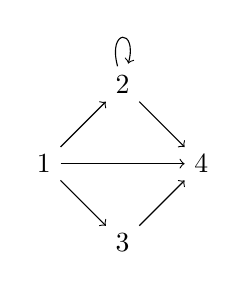
\begin{tikzpicture}
  \node(1)at(0,0){1};   \node(2)at(1,1){2};
  \node(3)at(1,-1){3};  \node(4)at(2,0){4};
  \draw[->] (1)edge(2)edge(3)edge(4) (2)edge(4)edge[loop above]() (3)edge(4);
\end{tikzpicture}}
~~~~~~~~~~~
\wrap[b]{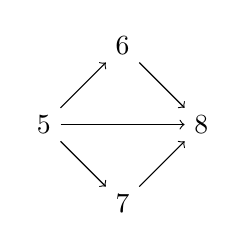
\begin{tikzpicture}
  \node(1)at(0,0){5};   \node(2)at(1,1){6};
  \node(3)at(1,-1){7};  \node(4)at(2,0){8};
  \draw[->] (1)edge(2)edge(3)edge(4) (2)edge(4) (3)edge(4);
\end{tikzpicture}}
\\[4mm]
\eg, (4) is the only world satisfying $\Box\bot$
\end{exampleblock}
%%%
% from ML for open minds
% 3: <>[]ff /\ [][]ff --- (also [][]ff?)
% 1: <>(3:)
% 2: <><>tt /\ not(1:)
% tip: last point as negation of all others...
% on the rhs: 2 becomes 3.
\end{frame}

%----------------------------------------------------------------------------------
\begin{slide}{Frame definability}\label{s:32}
\small
\begin{itemize}
  \item A modal formula is valid on a frame if it is true under \red{every valuation} at \red{every world} (i.e., it cannot be refuted)
  \item The class of frames defined by a modal formula $\phi$ are those where $\phi$ is valid.
  \item Example: $\eventual\eventual p \to \eventual p$ defines transitivity:\\
  ~~~~$\ger{F}=\pair{W,R}$ is transitive iff \red{for all $V$ and $w$},\\
  ~~~~$\pair{\ger{F},V},w\models \eventual\eventual p \to \eventual p $
\end{itemize}
\end{slide}
%----------------------------------------------------------------------------------
\begin{slide}{Exercise}\label{s:32}
\small

\begin{exampleblock}{Exercise: other properties}
\begin{enumerate}
  \item Transitivity: \dkb{$\eventual\eventual p \to \eventual p$}
  \item Reflexivity: \visible<2->{\dkb{$p \to \eventual p$}}
  \item Symmetry:    \visible<2->{\dkb{$p \to \always \eventual p$}}
  \item Confluence:  \visible<2->{\dkb{$\eventual\always p \to \always \eventual p$}}
  \item Irreflexibility:  \visible<2->{\alert{Not possible}}
\end{enumerate}
\end{exampleblock}

\end{slide}

%----------------------------------------------------------------------------------

\begin{slide}{Exercise}\label{s:32}
\small
\begin{exampleblock}{Bisimilarity and modal equivalence}
\begin{itemize}
\item Consider the following transition systems:
\begin{equation*}
%??????
\xymatrix{
%&&&\\
&&& 5 &\\
1 \ar@(ul,ur)[]  \ar[r] & 2 & \hspace{0.3cm} & 3 \ar[u] \ar[d]  \ar@/^/[r]   & 4 \ar@/^/[l]  \\
&&& 6 &
}
\end{equation*}
Give a modal formula that can be satisfied at point $1$ but not at $3$.
%[]([]false \/ <>[]false) - after any step it either deadlocks in one or 2 steps.
% book - Modalities and Multimodalities
% It is enough to see that (lhs) and (another irreflexive model) are bisimilar, although one is reflexive and the other not.
% IF irreflexivity were modally definable, the modal formula PSI which defines it would have to be invariant under bisimulations.
% BUT if PSI were to be true in (v-another-irr-model) then it would be true in (lhs) by the invariance lemma, which is impossible since (u-lhs) is a reflexive point.
\item Show that  \dgold{irreflexivity} is modally undefinable.
\\(\ie, no formula that characterises a irreflexive system)
\item Prove the invariance lemma.
\end{itemize}
\end{exampleblock}
\end{slide}

%----------------------------------------------------------------------------------
\begin{slide}{Invariance and definability}\label{s:33}
\small
To prove the converse of the invariance lemma requires passing to an \dgold{infinitary} modal language  with arbitrary (countable) conjunctions and disjunctions. Alternatively, and more usefully, it can be shown  for \dgold{finite} models:
\begin{block}{Lemma (modal equivalence implies bisimulation)}
\red{If} two points $w, w'$ from two finite models $\ger{M} = \pair{\pair{W, R}, V}$ and $\ger{M}' = \pair{\pair{W', R'}, V'}$ satisfy the same modal formulas,
\\
\red{then} there is a bisimulation $S \subseteq W \times W'$  such that $w S w'$.
 \end{block}
\end{slide}

%----------------------------------------------------------------------------------
\begin{slide}{Invariance and definability}\label{s:34}
\small
\begin{block}{Note}
\begin{itemize}
\item The result can be \dkb{weakened} to \dgold{image-finite} models.
\item Combining this result with the invariance lemma one gets the so-called \dkb{modal equivalence theorem} stating that, for image-finite models, bisimilarity and modal equivalence coincide. The result is also known as the \dkb{Hennessy-Milner theorem} who first proved it for process logics.
%\item the situation is similar to what happens in first-order logic: first-order formulas are invariant for \dgold{potential isomorphism}, but the converse only holds in a weak formulation: two models are potentially isomorphic iff they have the same complete theory in the \dgold{infinitary} first-order logic.
\end{itemize}
\end{block}

\begin{exampleblock}{Exercise}
\begin{itemize}
\item Give an example of modally equivalent states in different Kripke structures which fail to be bisimilar.
% infinite models: one modal formula satisfies 2 non-bisimilar (infinite) models
% m1: infinte branching of finite steps 0, 0-1, 0-1-2, 0-1-2-3,...
% m2: same as m1, but with an extra infinitly long branch
% For every point, 
% https://books.google.pt/books?id=ql_dBtNOOeAC&pg=PA63&lpg=PA63&dq=not+bisimilar+infinite&source=bl&ots=ONMAmSjJ2E&sig=XpHSBzXyjJ0TUmImDu1Eg8MFnd4&hl=en&sa=X&redir_esc=y#v=onepage&q=not%20bisimilar%20infinite&f=false
\end{itemize}
\end{exampleblock}
\end{slide}


%----------------------------------------------------------------------------------
\begin{slide}{Invariance and definability}\label{s:35}
\small

\begin{block}{Lemma (modal logic vs first-order)}
The following are equivalent for all first-order formulas $\phi(x)$ in one free variable $x$:
\begin{enumerate}
\item $\phi(x)$ is invariant for bisimulation.
\item $\phi(x)$ is equivalent to the standard translation of a basic modal formula.
 \end{enumerate}
  \end{block}
  
 Therefore:\\
 \dgold{the basic modal language corresponds to the fragment of their first-order correspondence language that is invariant for bisimulation}
\end{slide}


%----------------------------------------------------------------------------------
\begin{slide}{Invariance and definability}\label{s:36}
\small

\begin{itemize}
\item the basic modal language (interpreted over the class of all models) is computationally better behaved than the corresponding first-order language (interpreted over the same models)
\item ... but clearly less  expressive 
\end{itemize}

\begin{center}
\begin{tabular}{|c|c|c|c|}
\hline
 & model checking & satisfiability \\ \hline
 ML & PTIME & PSPACE-complete  \\
 FOL & PSPACE-complete & undecidable \\
 \hline
\end{tabular}
\end{center}

  
  \vspace{0.2cm}
 \dgold{What are the trade-offs? Can this better computational behaviour be lifted to more expressive modal logics? }
\end{slide}


%-------------------------------------------------------------------------------
\begin{slide}{mCRL2 - modal logic}
\newcommand{\expr}{\mathit{mod}}
\newcommand{\midd}{\,~|~\,}
\centering
\begin{block}{Syntax (simplified)}
\begin{align*}
  \phi =&~ \mcode{true} \midd \mcode{false} \midd
          \mcode{forall x:T.}\phi \midd \mcode{exists x.:T}\phi \\|&~
          \phi~OP~\phi \midd \mcode{!}\phi \midd
          \mcode{[$\structure{\expr}$]}\phi \midd \mcode{<$\structure{\expr}$>}\phi \midd \ldots
\\[3mm]
\structure{\expr} =&~ \dkb{\alpha} \midd \mcode{nil} \midd \expr\mcode{+}\expr \midd
        \expr\mcode{.}\expr \midd \expr\mcode{*} \midd \expr\mcode{+}
\\[1mm]
\dkb{\alpha} =&~ \mcode{a(d)} \midd \mcode{a|b|c} \midd
          \mcode{true} \midd \mcode{false} 
          \midd
          \alpha~OP~\alpha \midd \mcode{!}\alpha
          \\|&~
          \mcode{forall x:T.}\alpha \midd \mcode{exists x:T.}\alpha 
          \midd
          \ldots
\end{align*}
\end{block}
%~\\[2mm]
where $OP = \set{\mcode{&&},\mcode{||},\mcode{=>}}$ ~~and~~
$T = \set{Bool, Nat, Int, \ldots}$

\begin{exampleblock}{Example}
``\code{[true*.a]<b>true}'' means \emph{``whenever an \code{a} appears after any number of steps, it must be immediately followed by \code{b}''}. 
\end{exampleblock}
\end{slide}

%-------------------------------------------------------------------------------
\begin{slide}{mCRL2 toolset overview}
  \centering
  
  \includegraphics[width=\textwidth]{images/mcrl2-toolset.png}

  -- mCRL2 tutorial: Verification part --
\end{slide}



 \section{Temporal logic}


%----------------------------------------------------------------------------------
\begin{slide}{Richer modal logics}\label{s:40}
\small

can be obtained in different ways, e.g.

\begin{itemize}
\item axiomatic extensions
\item introducing more complex satisfaction relations
\item \dgold{support novel semantic capabilities}
\item ...
\end{itemize}
 
 Examples
 \begin{itemize}
 \item richer temporal logics
\item hybrid logic
 \item modal $\mu$-calculus 
\end{itemize}
\end{slide}


%----------------------------------------------------------------------------------
%\begin{slide}{Temporal logics with $\mathcal{U}$ and $\mathcal{S}$}\label{s:41}
%\small
%\begin{block}{Until and Since}
%\begin{align*}
%\ger{M}, w  &\models \phi\, \mathcal{U}\, \psi & \text{ ~~ \textsf{iff} ~~} &
%\text{there exists}\; v \in W \;\text{st}\; w R v\; \text{and}\; \ger{M}, v \models \psi,\\
%& & & \text{and for all}\; u\; \text{st}\; w R u\; \text{and}\; u R v,\; \text{one has}\;  \ger{M}, u \models \phi\\
%\ger{M}, w  &\models \phi\, \mathcal{S}\, \psi & \text{ ~~ \textsf{iff} ~~} &
%\text{there exists}\; v \in W \;\text{st}\; v R w\; \text{and}\; \ger{M}, v \models \psi,\\
%& & & \text{and for all}\; u\; \text{st}\; v R u\; \text{and}\; u R w,\; \text{one has}\;  \ger{M}, u \models \phi
%\end{align*}
%\end{block}
%%
%\begin{itemize}
%\item note the $\exists\, \forall$ qualification pattern: these operators are neither diamonds nor boxes.
%\item  more expressive --- e.g. helpful to express \dgold{guarantee} properties, 
%e.g. \dkb{some event will happen, and a certain condition will hold until then}
%\end{itemize}
%\end{slide}
%
%----------------------------------------------------------------------------------
\newcommand{\Until}{\mathop{\mathcal{U}}} 
\newcommand{\Since}{\mathop{\mathcal{S}}} 
\begin{frame}{Temporal Logics with $\Until$ and $\Since$}
\begin{block}{Until and Since}
  \begin{align*}
    \ger{M},w & \models \phi\Until\psi
      & \text{iff}~~& \text{there \gold{exists} $v$ st
                      $w\alert{\leq}v$ and $\ger{M},v \models \psi$, and} \\
      && & \text{\gold{for all} $u$ st $w \alert{\leq} u \alert{<} v$,
                 one has $\ger{M},u \models \phi$}
    \\[2mm]
    \ger{M},w & \models \phi\Since\psi
      & \text{iff}~~& \text{there \gold{exists} $v$ st
                      $v\alert{\leq}w$ and $\ger{M},v \models \psi$, and} \\
      && & \text{\gold{for all} $u$ st $v \alert{<} u \alert{\leq} w$,
                 one has $\ger{M},u \models \phi$}
  \end{align*}
\end{block}
%
\begin{itemize}
\item Defined for temporal frames $\pair{T,<}$ (transitive, asymmetric).
\item note the $\exists\, \forall$ qualification pattern: these operators are neither diamonds nor boxes.
\item  More general definition for other frames -- it becomes more expressive than modal logics.
\end{itemize}
\end{frame}

%----------------------------------------------------------------------------------
\begin{frame}{Exercise}
\begin{exampleblock}{Temporal logics - rewrite using $\Until$}
\begin{itemize}
  \item $\eventual \psi = \only<2->{\blue{tt \Until \psi}}$
  \item $\always \psi = \only<3>{\blue{\lnot(\eventual \lnot \psi)} = \blue{
                        \lnot(tt \Until \lnot\psi)}}$
\end{itemize}
\end{exampleblock}
  
\end{frame}


%\begin{slide}{Exercise}\label{s:42}
%\small
%\begin{exampleblock}{Temporal logics}
%\begin{itemize}
%\item Show that  $\mathcal{U}$ is modally undefinable.\\
%\emph{Hint} Consider the following transition structures and formula $\false\, \mathcal{U}\, \true$:
%
%\begin{equation*}
%%????????
%\xymatrix{
%%&&&\\
%1 \ar@(ul,ur)[]   & \hspace{0.3cm} & 2  \ar@/^/[r]   & 3 \ar@/^/[l]  
%}
%\end{equation*}
%\item Would this be the case if we restrict ourselves to transitive, irreflexive models?
%\end{itemize}
%\end{exampleblock}
%\end{slide}


%----------------------------------------------------------------------------------
\begin{slide}{Linear temporal logic (LTL)}\label{s:44}
\small

\[
\phi\, := \; \true \mid p \mid  \phi_1 \wedge \phi_2 \mid \neg \phi \mid \blue\nexts \phi \mid  \phi_1 \,\blue\Until\, \phi_2 %\mid \eventual \phi \mid \always \phi
\]
\vspace{0.5cm}
\begin{center}
\begin{tabular}{|l|c|}
\hline
mutual exclusion  & $\blue\always (\neg c_1 \vee \neg c_2)$ \\
 liveness & $\blue\always \blue\eventual c_1 \wedge \blue\always \blue\eventual c_2$\\
starvation freedom  & $(\blue\always \blue\eventual w_1 \impp \blue\always \blue\eventual c_1) \wedge
(\blue\always \blue\eventual w_1 \impp \blue\always \blue\eventual c_1)$ \\
progress & $\blue\always (w_1 \impp \blue\eventual c_1)$\\
weak fairness & $\blue\eventual \blue\always w_1 \, \impp \blue\always \blue\eventual c_1$\\
eventually forever & $\blue\eventual \blue\always w_1$\\
\hline
\end{tabular}  
\end{center}

\begin{itemize}
\item First temporal logic to reason about reactive systems [Pnueli, 1977]
\item Formulas are interpreted over \dkb{execution paths}
\item Express \dkb{linear-time properties}
\end{itemize}
\end{slide}

%----------------------------------------------------------------------------------
\begin{slide}{Computational tree logic (CTL, CTL*)}\label{s:45}
\small

 \dgold{state} formulas to express  properties of a state:
\[
\Phi\, := \; \true \mid \Phi \wedge \Phi \mid \neg \Phi \mid \dgold{\exists} \psi \mid \dgold{\forall} \psi
\]


\dkb{path} formulas to express properties of a path:
\[
\psi\, := \; \dkb{\nexts} \Phi \mid  \Phi \dkb{\until} \Psi
             %\mid \eventual \phi \mid \always \phi
\]

\vspace{0.2cm}
\begin{center}
\begin{tabular}{|l|c|}
\hline
mutual exclusion  & $\dgold{\forall} \dkb{\always} (\neg c_1 \vee \neg c_2)$ \\
 liveness & $\dgold{\forall} \dkb{\always} \forall \eventual c_1 \wedge \dgold{\forall} \dkb{\always} \dgold{\forall}  \dkb{\eventual} c_2$\\
order  & $\dgold{\forall} \dkb{\always} (c_1 \vee \dgold{\forall}\dkb{\nexts} c_2)$\\
\hline
\end{tabular}  
\end{center}

\begin{itemize}
\item Branching time structure encode transitive, irreflexive but not necessarily linear flows of time
\item flows are \dgold{trees}: past linear; branching future
\end{itemize}
\end{slide}


\section{Hybrid logic}
%----------------------------------------------------------------------------------
\begin{slide}{Hybrid logic}\label{s:46}
\small

\begin{block}{Motivation}
Add the possibility of \dgold{naming} points and reason about their \dgold{identity}

\vspace{0.5cm}
Compare:
\begin{equation*}
\eventual (r \e p)\; \e\; \eventual (r \e q)\; \; \impp\; \; \eventual (p \e q)
\end{equation*}
with
\begin{equation*}
\eventual (\alert{i} \e p)\; \e\; \eventual (\alert{i} \e q)\; \; \impp\; \; \eventual (p \e q)
\end{equation*}
for $\alert{i \in \mathsf{NOM}}$ (a \dgold{nominal})
\end{block}

\begin{block}{Syntax}
  \begin{equation*}
\phi\; ::=\;
    \ldots \:\mid\:
    \dgold{p} \: \mid\: 
    \dkb{\pv{m}{\phi}} \:  \mid\:
    \dkb{\nc{m}{\phi}} \:  \mid\:
    \alert{i} \:  \mid\:
    \alert{@_i}\,\phi
\end{equation*}
where $\dgold{p \in \mathsf{PROP}}$ and $\dkb{m \in \mathsf{MOD}}$ and $\alert{i \in \mathsf{NOM}}$
\end{block}
\end{slide}

%----------------------------------------------------------------------------------
\begin{slide}{Hybrid logic}\label{s:47}
\small

\begin{block}{Nominals $i$}
\begin{itemize}
\item Are special propositional symbols that hold exactly on one state (the state they \dkb{name})
\item  In a model the \dkb{valuation} $V$ is extended from 
$$ \fdec{V}{\mathsf{PROP}}{\pow{(W)}} $$
to
$$ \fdec{V}{\mathsf{PROP}}{\pow{(W)}} \; \; \; \text{and}\; \; \;  \dkb{\fdec{V}{\mathsf{NOM}}{W} }$$
where $\mathsf{NOM}$ is the set of nominals in the model
\item Satisfaction:
\begin{align*}
\alert{\ger{M}, w  \models  i} &&  \text{\textsf{iff} }  & w = V(i)
\end{align*}
\end{itemize}
\end{block}


\end{slide}



%----------------------------------------------------------------------------------
\begin{slide}{Hybrid logic}\label{s:48}
\small

\begin{block}{The $@_i$ operator}
\begin{align*}
\alert{\ger{M}, w \models  @_i \phi}
  &&  \text{~ \textsf{iff} ~~}  &\ger{M}, u  \models \phi\; \text{and $u = V(i)$ [$u$ is the state denoted by $i$]}
\end{align*}
\end{block}

\begin{block}{Standard translation to first-order}
\begin{align*}
ST_x(i) & =  (x = i)\\
ST_x(@_i \phi) & =  ST_i(\phi)[x \leftarrow i]\\
\end{align*}
i.e., hybrid logic corresponds to a first-order language enriched with constants and equality.
\end{block}
\end{slide}




%----------------------------------------------------------------------------------
\begin{slide}{Hybrid logic}\label{s:49}
\small

\begin{block}{Increased frame definability}
\begin{itemize}
\item \dgold{irreflexivity}: $i \impp \neg \eventual i$\\
\item \dgold{asymmetry}: $i \impp \neg \eventual \eventual i$\\
\item \dgold{antisymmetry}: $i \impp \always (\eventual i \impp i)$\\
\item \dgold{trichotomy}: $@_j \eventual i\; \ou\; @i_j    \; \ou\;   @_i \eventual j$
\end{itemize}
\end{block}

\end{slide}




%----------------------------------------------------------------------------------
\begin{slide}{Bisimulation with nominals}\label{s:50}
\small
\begin{block}{Definition}
Given two models $\ger{M} = \pair{\pair{W, R}, V}$ and $\ger{M}' = \pair{\pair{W', R'}, V'}$, a \dgold{bisimulation} is a non-empty binary relation
$S \subseteq W \times W'$  st whenever $w S w'$ one has that
\begin{itemize}
\item points $w$ and $w'$ satisfy the same propositional symbols \dkb{and nominals}
\item if $w R v$, then there is a point $v'$ in $\ger{M}'$ st  $w' R v'$ and $v S v'$ \hspace{0.3cm} (\dgold{zig})
\item if $w' R' v'$, then there is a point $v$ in $\ger{M}$ st  $w R v$ and $v S v'$ \hspace{0.3cm} (\dgold{zag})
\item \dkb{$V(i)\, R\, V'(i)$ for all nominal $i$} (\dgold{name consistency})
\end{itemize}
\end{block}

An \dkb{invariance} theorem and its \dkb{dual} (for image finite models) can also be proved

\end{slide}

%----------------------------------------------------------------------------------
\begin{slide}{Hybrid logic}\label{s:51a}
\small

\begin{block}{Summing up}
\begin{itemize}
\item basic hybrid logic is a simple notation for capturing  the \dgold{bisimulation-invariant fragment of first-order logic with constants and equality}, i.e., a mechanism for equality reasoning in propositional modal logic. 
\item comes \dgold{cheap}: up to a polynomial, the complexity of the resulting decision problem is no worse than for the basic modal language
\end{itemize}
\end{block}
\end{slide}

%----------------------------------------------------------------------------------
\begin{slide}{Hybrid logic}\label{s:51b}
\small


\begin{block}{Applications to architectural design}
\begin{itemize}
\item \dgold{layout of coordination circuits} (e.g. in \reo)
\item \dgold{reconfigurable architectures} (parametric on a specification logic)
\item \dgold{hierarchical architectures} (e.g. UML statecharts)
\item ...
\end{itemize}
\end{block}
\begin{flushright}
\dgold{[recent research at HASLab: projects \textsc{Dali} and \textsc{Nasoni}]}
\end{flushright}
\end{slide}

%----------------------------------------------------------------------------------
%\begin{slide}{Applications to architectural design}\label{s:52}
%\small
%
%\begin{block}{Structural reasoning over \reo circuits}
%
%$$
%\begin{array}{c}
%\phi\; :== \; p\; \mid i \: \mid\: \neg \phi \: \mid\: \phi_1 \land \phi_2\:  \mid\: \nc{K}{\phi} \:   \mid\:  \nco{K}{\phi} \:  \mid \: @_i \phi
%           %\pv{K}{\phi} \:  \mid\: \pvo{K}{\phi} \:  \mid\:
%\end{array}
%$$
%\begin{itemize}
%\item modalities are indexed by regular expressions over channel \dkb{types};
%\item $\pv{K}$ and $\nc{K}$ (reps., $\pvo{K}$ and $\nco{K}$) express properties of \dkb{outgoing} (resp., \dkb{incoming}) connections from the node in which they are evaluated.
%%\item @  \emph{redirects} the formula evaluation to the context of a specific node.
%%\item Nominals make possible to express proprieties \emph{local} to a specific node.
%\end{itemize}
%\end{block}
%\begin{flushright}
%\dgold{[Nuno Oliveira PhD thesis (MAP-i, 2015)]}
%\end{flushright}
%\end{slide}
%
%
%%----------------------------------------------------------------------------------
%\begin{slide}{Applications to architectural design}\label{s:53}
%\small
%
%\begin{block}{Structural reasoning over \reo circuits}
%
%\begin{center}
%
%\begin{tikzpicture}
%\ionode{(tout)}{(-0.5,1)}{node[left, xshift=-3pt]{\scriptsize $i$}}
%\ionode{(ho)}{(7,0)}{node[right, xshift=3pt]{\scriptsize $h_{o}$}}
%\mixednode{(j)}{(1,0)}{node[left, yshift=0, xshift=-3]{\scriptsize $j$}}
%\mixednode{(a)}{(3,0)}{node[below, yshift=0, xshift=6]{\scriptsize $a$}}
%\mixednode{(esi)}{(6,1)}{node[right, yshift=-5, xshift=0]{\scriptsize $es_i$}}
%\mixednode{(e)}{(3,1)}{node[left, yshift=0, xshift=-3]{\scriptsize $e$}}
%\xrouter{(xr1)}{(6,0)}{}
%\xrouter{(xr2)}{(1,1)}{}
%
%\sync{(tout)}{(xr2)}{
%	node[above, yshift=-1, xshift=12]{\scriptsize $y_i$}
%	node[above, yshift=1, xshift=29]{\scriptsize $y_{1}$}
%	node[below, yshift=-1, xshift=29]{\scriptsize $y_{2}$}
%}
%
%\Uchannel{sync}{(xr2)}{(esi)}{0.8}{v}{+}{}
%\sync{(xr2)}{(j)}{}
%
%\fifoe{(j)}{(a)}{
%		node[above, yshift=3pt, xshift=-17]{\scriptsize $w$}
%	}
%
%\fifoe{(a)}{(xr1)}{
%	node[above, yshift=3, xshift=-27]{\scriptsize $MAs$}
%	node[below, yshift=1, xshift=8]{\scriptsize $x_i$}
%	node[above, yshift=2, xshift=13]{\scriptsize $x_{1}$}
%	node[below, yshift=1, xshift=29]{\scriptsize $x_{2}$}
%}
%\sync{(xr1)}{(esi)}{}
%\sync{(xr1)}{(ho)}{}
%
%\fifoe{(esi)}{(e)}{node[above, yshift=3pt, xshift=25]{\scriptsize $Es$}}
%\sync{(e)}{(a)}{}
%\end{tikzpicture}
%\end{center}
%
%
%\begin{enumerate}
%\item \dkb{$\phi_1 \deff \ @_{t_o} \pv{-^*}{\true} \e \nc{-^{*}}\nc{-MAs}{\false}$}  \\
%(there is a path from triage input port ($t_{o}$) to a $MAs$ edge)
%\item \dkb{$\phi_2 \deff  \nco{-}\false \impp   \nc{-^*}h_o$}\\
%(all paths from input ports, lead to the billing service ($h_{o}$) port)
%\end{enumerate}
%
%\end{block}
%\end{slide}
%
%
%
%%----------------------------------------------------------------------------------
%\begin{slide}{Applications to architectural design}\label{s:54}
%\small
%\vspace{0.2cm}
%\begin{block}{Reconfiguration of \reo circuits}
%\begin{minipage}[b]{0.45\linewidth}
%\begin{center}
%
%%\emph{(a)}
%
%\begin{tikzpicture}
%\ionode{(a)}{(0,1.5)}{node[left, xshift=-3pt]{\scriptsize $\node{a}$}}
%\ionode{(b)}{(0,0.5)}{node[left, xshift=-3pt]{\scriptsize $\node{b}$}}
%
%\mixednode{(c)}{(0.8,1)}{node[below, yshift=-3pt]{\scriptsize $\node{cde}$}}
%\mixednode{(d)}{(1.7,1)}{node[below, yshift=-3pt]{\scriptsize $\node{fgh}$}}
%
%\ionode{(e)}{(2.5,1.5)}{node[right, xshift=3pt]{\scriptsize $\node{i}$}}
%\ionode{(f)}{(2.5,0.5)}{node[right, xshift=3pt]{\scriptsize $\node{j}$}}
%
%\fifoe{(a)}{(c)}{}
%\sync{(b)}{(c)}{}
%
%\sync{(c)}{(d)}{}
%\lossysync{(d)}{(e)}{}
%\lossysync{(d)}{(f)}{}
%
%\end{tikzpicture}
%
%\end{center}
%\end{minipage}
%\hspace{0.2cm}
%\begin{minipage}[b]{0.45\linewidth}
%\begin{center}
%
%%\emph{(b)}
%
%\begin{tikzpicture}
%\ionode{(a)}{(0,1.5)}{node[left, xshift=-3pt]{\scriptsize $\node{a}$}}
%\ionode{(b)}{(0,0.5)}{node[left, xshift=-3pt]{\scriptsize $\node{b}$}}
%
%\ionode{(ac)}{(1,1.5)}{node[right, xshift=3pt]{\scriptsize $\node{c}$}}
%\ionode{(bc)}{(1,0.5)}{node[right, xshift=3pt]{\scriptsize $\node{d}$}}
%\ionode{(cd)}{(2,1)}{node[left, xshift=-3pt]{\scriptsize $\node{e}$}}
%
%\mixednode{(d)}{(2.7,1)}{node[below, yshift=-3pt]{\scriptsize $\node{fgh}$}}
%
%\ionode{(e)}{(3.5,1.5)}{node[right, xshift=3pt]{\scriptsize $\node{i}$}}
%\ionode{(f)}{(3.5,0.5)}{node[right, xshift=3pt]{\scriptsize $\node{j}$}}
%
%\fifoe{(a)}{(ac)}{}
%\sync{(b)}{(bc)}{}
%
%\sync{(cd)}{(d)}{}
%\lossysync{(d)}{(e)}{}
%\lossysync{(d)}{(f)}{}
%
%\end{tikzpicture}
%
%\end{center}
%\end{minipage}
%
%
%\begin{minipage}[b]{\linewidth}
%\begin{center}
%
%\begin{tikzpicture}
%\ionode{(a)}{(-1,1)}{node[left, xshift=-3pt]{\scriptsize $\node{a}$}}
%\ionode{(b)}{(-1,0)}{node[left, xshift=-3pt]{\scriptsize $\node{b}$}}
%
%\mixednode{(mi)}{(-0.1,0.5)}{node[below, xshift=8pt]{\scriptsize $\node{cdm_i}$}}
%%\mixednode{(bc)}{(0,0)}{node[below, xshift=3pt]{\scriptsize $bc$}}
%\mixednode{(mo)}{(1.1,0.5)}{node[below, xshift=8pt]{\scriptsize $\node{m_oe}$}}
%
%\mixednode{(d)}{(2,0.5)}{node[below, yshift=-3pt]{\scriptsize $\node{fgh}$}}
%
%\ionode{(e)}{(3,1)}{node[right, xshift=3pt]{\scriptsize $\node{i}$}}
%\ionode{(f)}{(3,0)}{node[right, xshift=3pt]{\scriptsize $\node{j}$}}
%
%\fifoe{(a)}{(mi)}{}
%\sync{(b)}{(mi)}{}
%
%\sync{(mo)}{(d)}{}
%\lossysync{(d)}{(e)}{}
%\lossysync{(d)}{(f)}{}
%
%\path[-]
%	 (0,0) edge[bend left]  (0,0.5) 
%	 (0,0.5) edge [bend left] (0,1)
%	 (0,1) edge [bend left] (0.33, 1)
%	 (0.33,1) edge [bend left] (0.66, 1)
%	 (0.66,1) edge [bend left] (1, 1)
%	 (1,1) edge [bend left] (1, 0.5)
%	 (1,0.5) edge [bend left] (1, 0)
%	 (1,0) edge [bend left] (0.66,0)
%	 (0.66,0) edge [bend left] (0.33,0)
%	 (0.33,0) edge [bend left] (0,0)
%	 ;	 
%
%\end{tikzpicture}
%
%%\emph{(c)}
%
%\end{center}
%\end{minipage}
%
%\vspace{0.4cm}
%Invariant \dkb{$\Phi = \pv{\mathsf{sync}}{(\pv{-}{\true} \e \nc{-\mathsf{lossy}}{\false})}$} is \dkb{displaced} along a reconfiguration:
%$$
%\dkb{@_{\node{cde}}\, \Phi\; \; \leadsto \; \; @_{\node{m_oe}}\, \Phi}
%$$
%\end{block}
%\end{slide}
%
%
%%----------------------------------------------------------------------------------
%\begin{slide}{Applications to architectural design}\label{s:55}
%\small
%
%\begin{block}{Specifying reconfigurable architectures}
%\begin{itemize}
%\item Reconfigurable architectures are represented as \dkb{structured transition systems} whose
%\item states are endowed with  \dkb{local} specifications and
%\item  the \dkb{global} transition structure models system's evolution  through possible configurations.
%\item The hybrid language is developed \dkb{on top} whichever logic is taken for the local configurations (\eg, equational, first-order, fuzzy, etc.) \\
%--- by \dkb{hybridisation}.
%\end{itemize}
%\end{block}
%
%
%\begin{flushright}
%\dgold{[Alexandre Madeira PhD thesis (MAP-i, 2013)]}
%\end{flushright}
%\end{slide}
%
%%----------------------------------------------------------------------------------
%\begin{slide}{Applications to architectural design}\label{s:56}
%\small
%
%\begin{minipage}[b]{0.4\linewidth}
%  \centering
% \includegraphics[width=.8\linewidth]{images/HT-ex1.pdf}
%\end{minipage}
%\quad
%\begin{minipage}[b]{0.5\linewidth}
%  \centering
%  \includegraphics[width=.9\linewidth]{images/HT-ex2.pdf}
%\end{minipage}
%~\\
%
%\begin{itemize}
%\item $\mathcal{H}$: \gold{pure hybrid formulas}
%\item $\mathcal{H}^2$: \gold{hierarchical sturctures}, e.g. $$@_{j^1} k^0 \wedge^1 [\lambda^1] (\rho_1,\dots,\rho_n)$$
%\end{itemize}
%
%\end{slide}
%
%
%%----------------------------------------------------------------------------------
%\begin{slide}{Applications to architectural design}\label{s:57}
%\small
%
%\vspace{0.3cm}
%
%\begin{block}{Hierarchical  architectures}
%\begin{itemize}
%\item Hierarchical  architectures are represented as \dkb{hierarchical  transition systems} whose
% states are transition systems themselves 
%\item and (intrusive)  transitions between designated states in different local transition systems at different levels of abstraction are allowed.
%\item  Hybrid logic captures this principle which is inherent to well known design formalisms such as  statecharts and  UML.
%\end{itemize}
%\end{block}
%\vspace{-0.2cm}
%\begin{center}
%  \includegraphics[width=0.5\textwidth]{images/intro2.pdf}
%\end{center}
%
%\end{slide}



\end{document}
%%%%%%%%%%%%%%%%%%%%%%%%%%%%%%%%%%%%%%%%%%%%%%%%%%%%%%%%%%%%%%%%%%%%%%%%%%%%%%%%%%%



